\chapter{蛋白尿}

蛋白尿是肾脏疾病的常见临床表现,而全身性疾病亦可表现为蛋白尿。血液流经肾脏时由于正常肾小球毛细血管壁的电荷和孔径屏障,阻挡了血液中高分子量的蛋白质通过,因此原尿中只有少量白蛋白和球蛋白片段,而且流经近端肾小管过程中又几乎被肾小管上皮细胞重吸收。虽然正常肾小管和尿路也分泌少蛋白,但多数健康成人尿蛋白排泄总量<150mg/24h,蛋白质定性检查时,呈阴性反应。当尿中蛋白质含量>150mg/24h或尿蛋白/肌酐>200mg/
g,或尿常规检查尿蛋白定性试验阳性,称为蛋白尿(proteinuria)。如果尿蛋白含量≥3.5g/
24h,则称为大量蛋白尿。

\section{【蛋白尿的发生机制】}

1.肾小球滤过屏障受损 肾小球滤过膜的孔径屏障或电荷屏障受损,系膜细胞调节功能受损和肾小球血流动力学的改变,使肾小球滤过膜通透性增高,导致血浆蛋白漏入肾小囊腔,超过肾小管重吸收能力而形成蛋白尿。

2.肾小管的重吸收功能障碍,使肾小球滤过的小分子量蛋白不能被近曲小管充分重吸收而产生的蛋白尿。

3.肾和尿路排泌的蛋白质增多。

4.血中异常蛋白增多,经肾小球滤出,超过肾小管的重吸收能力而产生的蛋白尿。

\section{【蛋白尿的分类】}

根据蛋白尿的发生机制可分为肾小球性蛋白尿、肾小管性蛋白尿、混合性蛋白尿、溢出性蛋白尿和组织性蛋白尿。

\subsection{(一)肾小球性蛋白尿}

由于肾小球滤过屏障受损所致。此类蛋白尿的特点是尿蛋白含量较多,常>2g/24h;以白蛋白为主,可含有少量大分子量蛋白。根据病变滤过膜损伤的程度及尿蛋白组分又分为两种:①选择性蛋白尿:尿蛋白以白蛋白为主,并有小量小分子量蛋白,无大分子量蛋白(IgG、IgA、IgM和C3),定性(+++)~(++++),多见于微小病变,治疗反应较好;②非选择性蛋白尿:反映肾小球毛细血管壁有严重的损伤断裂,尿蛋白呈血浆蛋白成分,有大分子量蛋白(如IgG、IgM和C3)、中分子量蛋白(如白蛋白)和小分子量蛋白(如β\textsubscript{2}
-微球蛋白),定性(+)~(++++),可见于其他各型肾小球肾炎,治疗反应不佳,预后不良。

临床上可见于:①生理性:可由剧烈运动、高温作业、严重受寒、长期直立等因素,使肾血管痉挛或充血,导致肾小球滤过膜通透性增加而发生。②病理性:可见于各种原发或继发性肾小球疾病;蛋白尿的程度与病变部位和性质有关,而尿蛋白量的多少不能反映肾脏病变程度和预后。

\subsection{(二)肾小管性蛋白尿}

由于肾小管重吸收功能障碍所致。此类蛋白尿的特点是尿蛋白量较少,定量常为1~2g/24h,一般不超过2.0g/24h;以小分子量蛋白(如溶菌酶、β2-微球蛋白)为主,白蛋白含量较少,定性(+)~(++)。

临床上可见于:①小管间质病变:如间质性肾炎、肾盂肾炎、遗传性肾小管疾病。②中毒性肾间质损害:如重金属、有机溶剂或药物等引起的肾损害。③中草药如马兜铃、关木通等引起的肾损害。

\subsection{(三)混合性蛋白尿}

肾小球和肾小管同时受损,导致尿中出现小分子量和大分子量蛋白质。

临床上可见于:①各种原因所致的小管间质疾病,先侵犯肾小管,后累及肾小球,使两者均受累,如肾盂肾炎、间质性肾炎等。②各种肾小球疾病后期,先侵犯肾小球,后累及肾小管,使两者均受累,如慢性肾炎、肾移植排斥反应等。③全身性疾病同时侵犯肾小球和肾小管,如狼疮性肾炎、糖尿病肾病等。

\subsection{(四)溢出性蛋白尿}

由于血浆中异常蛋白如免疫球蛋白轻链、游离血红蛋白、肌红蛋白或溶菌酶、淀粉酶等增加所致。此类尿蛋白定量0.2~10g/24h,定性为(+)~(++),可出现免疫球蛋白轻链或本-周蛋白。

临床上可见于:①浆细胞病,如多发性骨髓瘤、巨球蛋白血症、重链病和轻链病,体内产生过多Ig轻链。②急性血管内溶血,如阵发性睡眠性血红蛋白尿时尿中出现血红蛋白。③大面积肌肉损伤、炎症,如挤压综合征、横纹肌溶解综合征时尿中出现肌红蛋白。④其他:如急性白血病时尿中出现溶菌酶,胰腺炎时尿淀粉酶增高;极个别的人,食进过多机体不能利用的蛋白质而从肾小球溢出,而造成“食物性蛋白尿”。

\subsection{(五)组织性蛋白尿}

由于肾小管、下尿路分泌的蛋白或其他蛋白质渗入尿中所致。此类尿蛋白含量一般不多,定性常为(±)~(+),定量可为0.5~1g/24h。

临床上可见于:远端肾小管分泌的Tamm-Horsfall蛋白,尿路上皮分泌的IgA,尿路感染产生的脓、血和分泌物中的黏蛋白以及前列腺液或精液等混入尿中等。

此外,蛋白尿还有其他分类方法,如根据蛋白尿持续的时间分为一过性蛋白尿和持续性蛋白尿。根据尿蛋白量的多少分为轻度蛋白尿(<1.0g/24h尿)、中度蛋白尿(1.0~3.5g/24h尿)和重度蛋白尿(>3.5g/24h尿)。根据蛋白尿的性质分为生理性蛋白尿(包括功能性蛋白尿和体位性蛋白尿或直立性蛋白尿)和病理性蛋白尿。本章内容主要是按蛋白尿性质的分类(表\ref{tab37-1})进行论述。

\section{【诊断步骤】}

\subsection{(一)确定是否是真性蛋白尿}

当常规尿蛋白定性检查阳性时应首先注意排除以下可能引起假阳性的情况:①尿中混有血液和脓液,此时尿标本在沉渣中可见到多量红细胞或白细胞、扁平上皮细胞,离心沉淀或过滤后,蛋白定性检查会转为阴性;②高度浓缩尿(尿比重>1.025);③强碱性尿(尿pH>8.0);④X线造影剂、青霉素类、头孢菌素类、磺胺类、甲苯磺丁脲、甲苯酰吡酸和盐酸偶苯氮吡胺等药物所致;⑤防腐剂如氯己定溶液(洗必泰)、苯扎溴铵溶液(新洁尔灭);⑥下尿路蛋白尿:患者有下尿路疾病表现,尿沉渣中无管型,如发现较多扁平上皮细胞、精子等,则可确定蛋白质是来自下尿路。

\begin{table}[htbp]
\centering
\caption{蛋白尿疾病的分类}
\label{tab37-1}
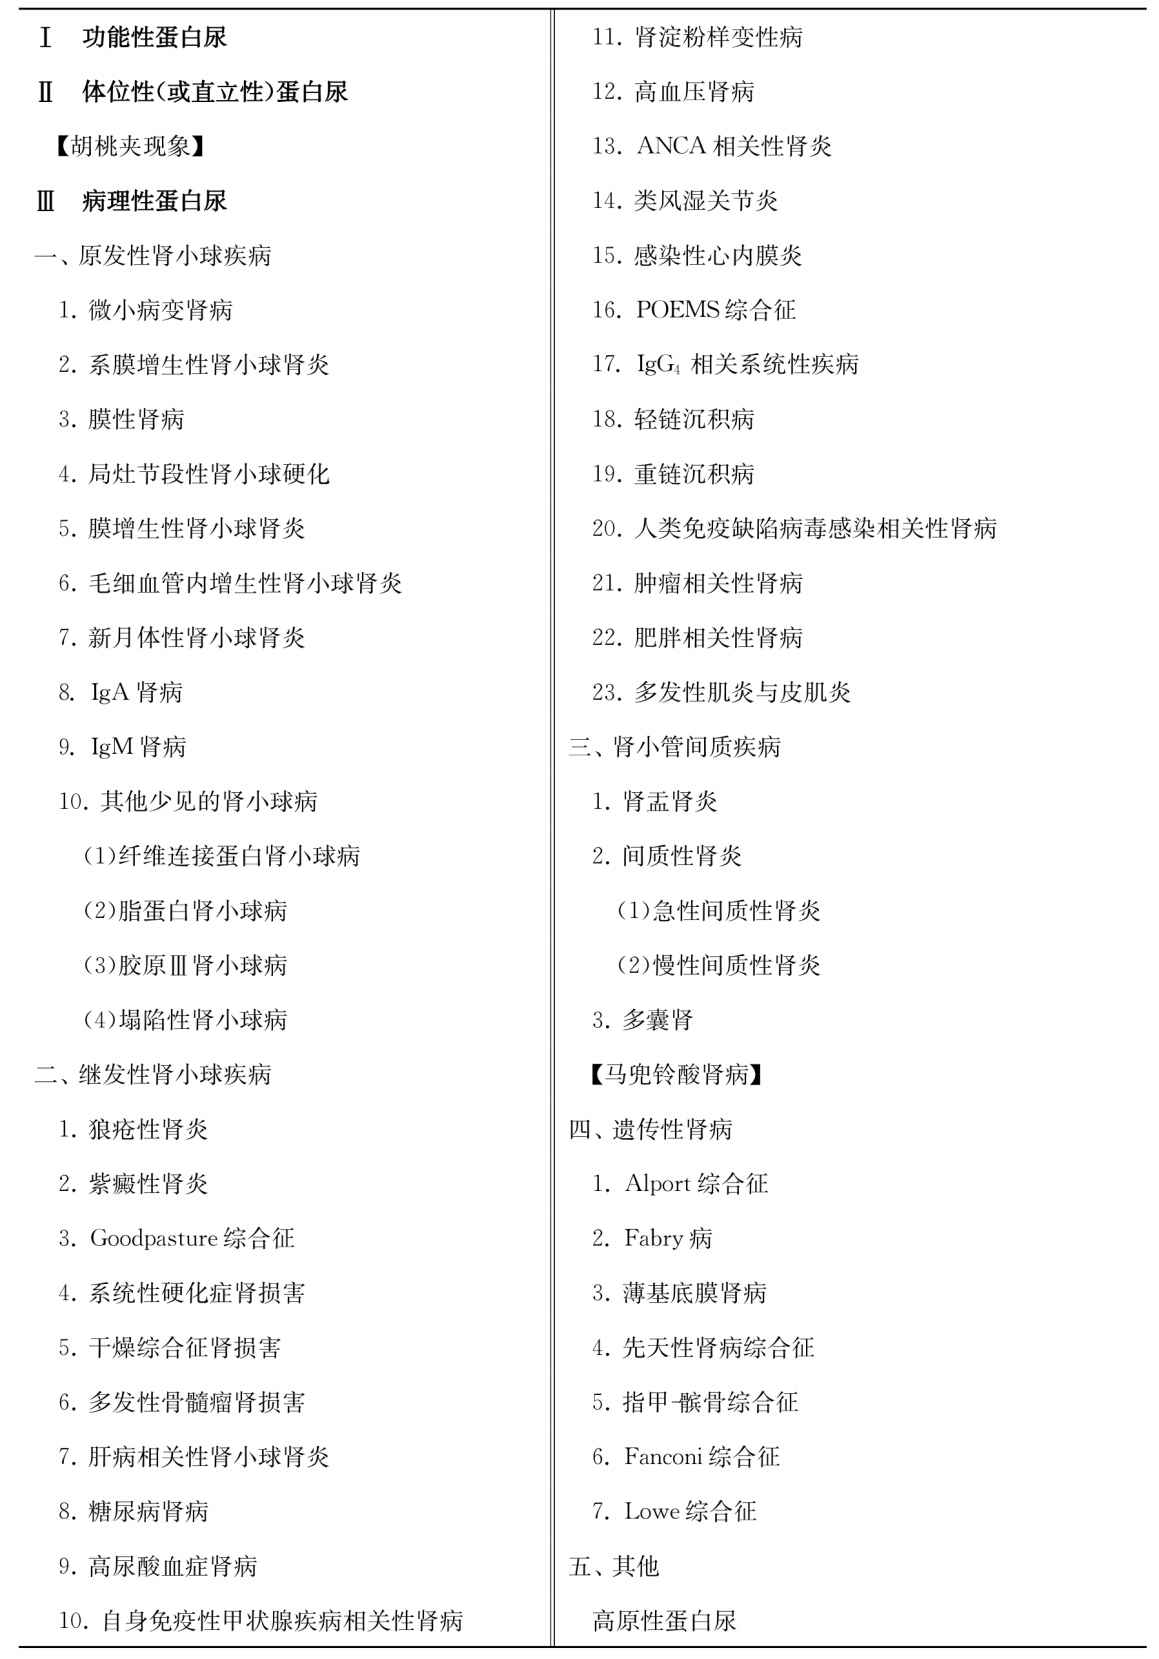
\includegraphics[width=5.97917in,height=8.5625in]{./images/Image00232.jpg}
\end{table}

\subsection{(二)判定蛋白尿是生理性还是病理性}

确定真性蛋白尿后,其次应除外生理性蛋白尿(即功能性蛋白尿和体位性蛋白尿)。功能性蛋白尿有一定的原因,如发热、受冻、剧烈运动、高温作业、应激状态、右心功能不全等;体位性蛋白尿,与体位改变有密切关系;两者均为暂时性,原因去除后,蛋白尿亦消失。如蛋白尿呈持续性,则不论其尿蛋白量多少,均应视为病理性。

\subsection{(三)确定病理性蛋白尿的组分和分子量}

肯定为病理性蛋白尿后,可行尿蛋白SDS盘状电泳,以判断蛋白尿是低分子量、中分子量、高分子量还是混合型蛋白尿。低分子量蛋白尿,主要电泳区带在白蛋白及白蛋白以下,提示为肾小管性或溢出性蛋白尿。中分子量蛋白尿,主要电泳区带在白蛋白上下;高分子量蛋白尿,主要电泳区带在白蛋白及白蛋白以上;中高分子量蛋白尿提示为肾小球性蛋白尿。混合型蛋白尿,尿蛋白主要以白蛋白区带为主,但在白蛋白以上及以下均有分布,提示肾小球及肾小管均受累。

\subsection{(四)确定病理性蛋白尿的病因}

对于低分子量蛋白尿,应注意检测血清球蛋白和某些特定蛋白浓度或行血清蛋白电泳以区分溢出性蛋白尿还是肾小管性蛋白尿。如为溢出性蛋白尿,应行有关浆细胞病、溶血、肌病和白血病等检查,必要时行骨髓穿刺术。如为肾小球性、肾小管性和混合性蛋白尿,应行肾脏病的相关检查,必要时行肾活检。

\protect\hypertarget{text00289.html}{}{}

\section{123 功能性蛋白尿}

功能性蛋白尿是一种轻度、暂时性、良性蛋白尿,原因去除后尿蛋白质能迅速消失。此种蛋白尿主要是由于体内或体外某些因素刺激肾脏,使肾血管痉挛或充血,血pH下降,增加肾小球滤过膜通透性所致。临床特点:①蛋白尿的主要成分为白蛋白;②24小时尿蛋白含量一般为0.5g以下,甚少超过1g;③常发生于健康青年或成年;④原因去除后尿蛋白阴转;⑤可见于剧烈体力劳动或运动后、长途行军期间、高温作业或严重受寒、精神紧张后等,发热病的极期、充血性心力衰竭也常产生此种蛋白尿,进食高蛋白饮食后所出现的蛋白尿也属此类。据报道,室外高温作业人员尿蛋白阳性率为9.74\%,招飞体检青年运动后蛋白尿发生率分别为81.95\%和79.54\%。此种蛋白尿需与原有的肾脏病,因运动、发热等使蛋白尿加重的情况相鉴别。

\protect\hypertarget{text00290.html}{}{}

\section{124 体位性(或直立性)蛋白尿}

体位性(或直立性)蛋白尿的发生与体位改变密切相关。临床特点:①清晨尿无蛋白质,起床活动后渐出现蛋白尿,长时间直立、行走或加强脊柱前凸姿势时,尿蛋白含量增多,平卧休息1小时后尿蛋白含量减少或消失;②多发生于瘦长体型的健康青年或成人,多数认为在青少年的发生率约为2\%~10\%;③24小时尿蛋白一般小于1g,偶可达2~3g,属非选择性蛋白尿,但卧位12小时尿蛋白总量应小于75mg;④无任何与肾脏有关的疾病的表现,肾功能正常,健康情况良好;⑤一般预后良好。

据报道,83例体位性蛋白尿患者随访5~10年,81\%患者尿蛋白自然消失,19\%患者发展为持续性蛋白尿或伴发作性血尿。另报道,116例体位性蛋白尿患儿随访5~18年,93例(80.2\%)尿蛋白消失,17例发展为持续性蛋白尿(其中3例出现肾功能损害,肾活检结果示:11例无异常,3例为微小病变肾病,2例为系膜增殖性肾炎,1例为局灶硬化型),6例转为间歇性蛋白尿伴发作性血尿(其中4例肾活检结果显示:3例无异常,1例为系膜增生性肾炎)。

因此,一般认为,对一些反复体位性蛋白尿,且常伴有血尿、管型尿或其他表现的患者,则应注意存在肾病的可能,应密切观察。

\subsection{附:胡桃夹现象}

胡桃夹现象又称左肾静脉压迫综合征,是因主动脉和肠系膜上动脉挤压左肾静脉所致。临床表现为无症状性直立性蛋白尿,发作性(或持续性)肉眼或镜下血尿,腹痛及精索静脉曲张。国内报道258例诊断为胡桃夹现象的儿童中,表现为非肾小球性血尿有109例(42.2\%),直立性蛋白尿有108例(41.8\%),非肾小球性血尿伴直立性蛋白尿8例,肾小球性血尿伴(或)持续性蛋白尿33例。

\protect\hypertarget{text00291.html}{}{}

\section{125 病理性蛋白尿}

病理性蛋白尿的特点:①蛋白尿持续存在,尿中蛋白含量较多;②常合并有其他尿检异常,如血尿、白细胞尿、管型尿等;③常伴有肾脏病的其他表现,如高血压、水肿等或全身性疾病的原发表现。

病理性蛋白尿主要见于各种原发性和继发性肾小球疾病、肾小管间质疾病、遗传性肾病、肾血管疾病和其他肾脏病(如妊娠性肾病、放射性肾病和移植肾病)等。本节将重点阐述临床上引起蛋白尿的常见疾病。

\subsection{一、原发性肾小球疾病}

国内报道原发性肾小球疾病病例占肾活检病例的70.58\%,男女比例为1.73∶1。本病病理类型多样(表\ref{tab37-2}),临床表现各异(表\ref{tab37-3})。\footnote{NS:肾病综合征;Uab:尿检异常;ANS:急性肾炎综合征;ARF:急性肾衰竭;RPGN:急进性肾炎综合征;CRF:慢性肾衰竭;HT:高血压;iGH:孤立性肉眼血尿;rGH:反复发作性肉眼血尿;MCD:微小病变肾病;MsP:系膜增生性肾炎;MN:膜性肾病;FSGS:局灶节段性肾小球硬化;MPGN:膜增生性肾炎;EnPGN:毛细血管内增生性肾炎;CREGN:新月体性肾炎;IgAN:IgA肾病;IgMN:IgM肾病}

\begin{table}[htbp]
\centering
\caption{原发性肾小球疾病的病理分型(参照WHO标准)}
\label{tab37-2}
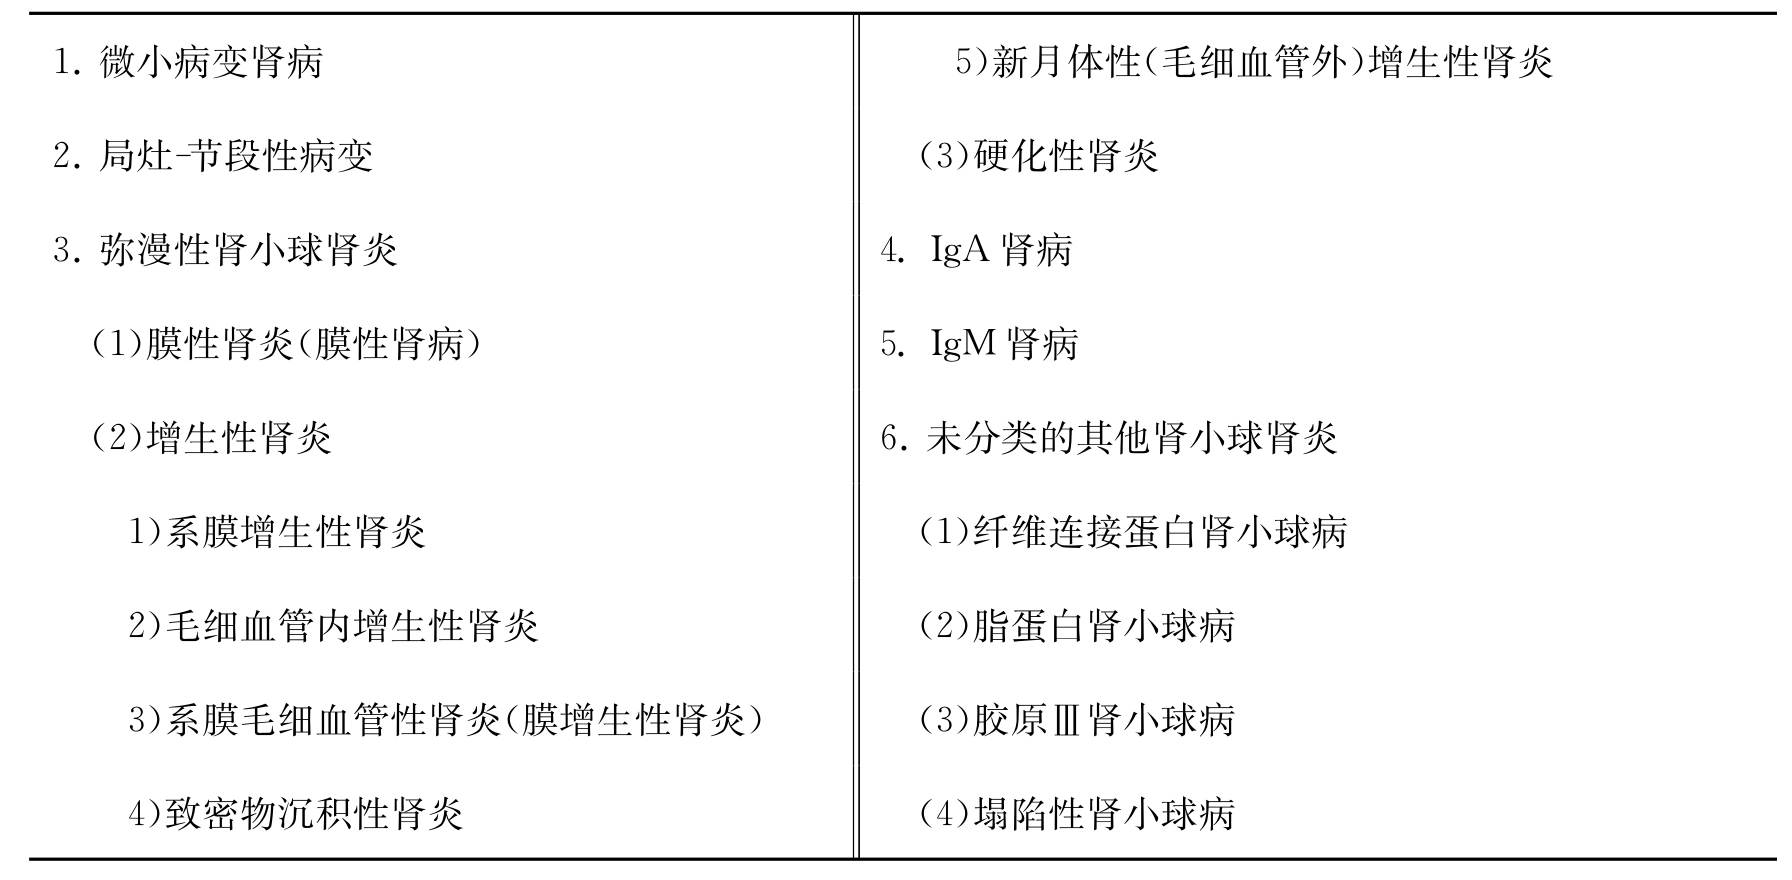
\includegraphics[width=5.96875in,height=2.92708in]{./images/Image00233.jpg}
\end{table}

\begin{table}[htbp]
\centering
\caption{原发性肾小球疾病各病理类型的临床表现(\%)}
\label{tab37-3}
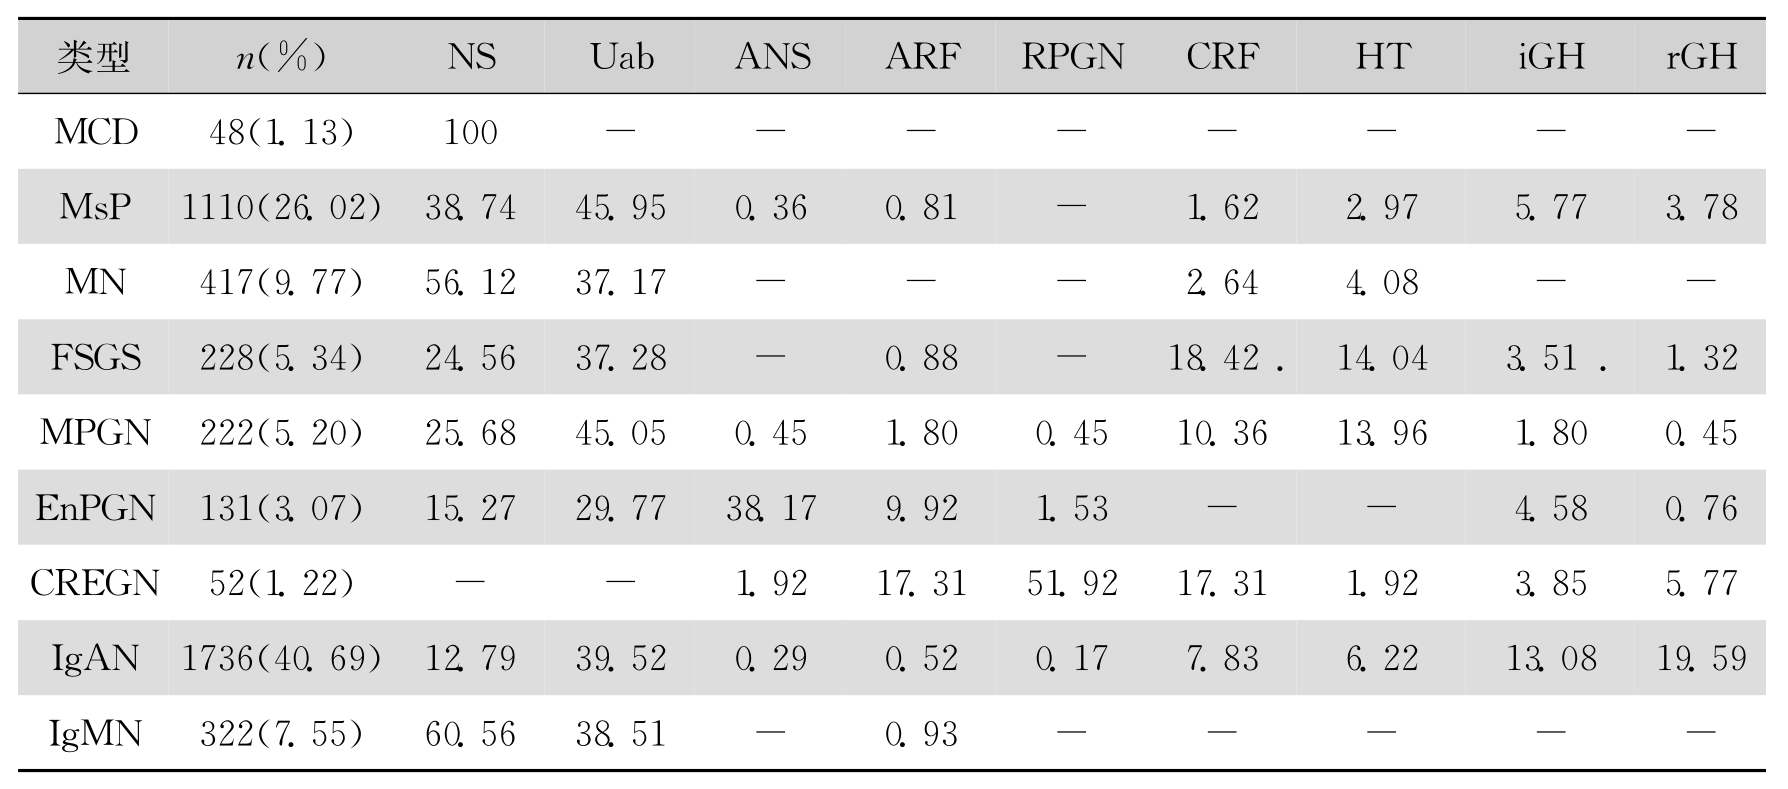
\includegraphics[width=5.94792in,height=2.61458in]{./images/Image00234.jpg}
\end{table}

\subsubsection{(一)微小病变肾病(minimal change disease,MCD)}

MCD是肾病综合征的常见病理类型。好发于儿童,儿童男多于女,成人男女差别不明显。大部分无任何诱因而突然起病,也有部分有上呼吸道感染或过敏史。水肿为常见和首发的症状,一般无血尿,少数可有镜下血尿,高血压较少见。多见于成年人。

国内报道4298例成年肾小球疾病患者,MCD占原发性肾小球疾病的2.3\%,其中男女比例为2.75∶1,年龄分布主要在15~34岁(占85.4\%)。另报道MCD在婴幼儿和老年人原发性肾小球疾病的比例分别为29.1\%和2.6\%。

\subsubsection{(二)系膜增生性肾小球肾炎(mesangial proliferative}
glomerulonephritis,MsPGN)

MsPGN是一组以光镜下肾小球呈弥漫性系膜细胞增生和(或)系膜基质增多,而毛细血管壁正常为特征的肾小球性肾炎。根据系膜区免疫球蛋白沉积的不同,可分为IgA肾病和非IgA系膜增生性肾小球肾炎。这里论述的是非IgA系膜增生性肾小球肾炎。MsPGN是原发性肾小球疾病的常见病理类型之一。好发于青少年,男性居多。临床表现多样,可表现为无症状性蛋白尿、孤立性血尿、蛋白尿合并血尿、肾病综合征和慢性肾炎,此外尚有高血压和肾功能减退。

国内报道MsPGN占原发性肾小球疾病的比例,婴幼儿为49.5\%,成人为29.7\%,老年人为35.1\%。

\subsubsection{(三)膜性肾病(membranous nephropathy,MN)}

MN是成人原发性肾病综合征的常见病理类型。多见于成人,男多于女。多隐匿起病,少数有前驱感染。绝大多数呈大量蛋白尿,为非选择性蛋白尿;镜下血尿少见,一般无肉眼血尿;早期血压多正常,随病程进展,可有半数出现高血压;早期肾功能多正常,少数可逐渐出现肾功能不全、尿毒症。肾静脉血栓发生率较高(约50\%)。

国内报道,MN在原发性肾小球疾病中占9.5\%,在婴幼儿、成人和老年人中的比例分别为1.0\%、8.8\%和39.0\%,而在老年人肾病综合征中占44\%。另报道在老年人原发性肾病综合征中MN占28.57\%~30.43\%。一组214例成人MN病例中,发病年龄主要在21~50岁(71.0\%),男女比例为2.75∶1,临床表现为大量蛋白尿(29.9\%)、高血压(14.0\%)、肾功能不全(6.1\%)及镜下血尿(41.6\%),23.8\%的患者表现为肾病综合征,随访中16.2\%患者发生肾功能恶化。

\subsubsection{(四)局灶节段性肾小球硬化(focal segmental glomerulosclerosis,FSGS)}

FSGS是原发性肾病综合征的常见病理类型。好发于儿童和青少年,男性多见。多隐匿起病,少数发病前有上呼吸道感染或过敏史。常见临床表现为肾病综合征,可有部分为非肾病性蛋白尿,尿蛋白为非选择性;镜下血尿常见,可有肉眼血尿;肾功能损害可见于初诊者,但多在病程中逐渐出现;常有肾小管功能损害表现;高血压多见。

国内报道,FSGS在原发性肾小球疾病中占5.8\%,在婴幼儿、成人和老年人的比例分别为1.0\%、5.6\%和5.2\%。有报道114例原发性FSGS患者,男女比例为1.48∶1,表现为蛋白尿(93.0\%,其中肾病综合征21.9\%),血尿(51.8\%,肉眼血尿14.9\%,镜下血尿36.8\%),高血压(43.8\%),肾功能不全者(47.4\%),随访中22.2\%发展至尿毒症。另报道38例FSGS患儿,男女之比为1.92∶1,表现为蛋白尿(100\%,其中肾病综合征占89.5\%),血尿(63.2\%,肉眼血尿13.2\%),高血压(28.9\%),肌酐清除率降低(18.4\%)。

\subsubsection{(五)膜增生性肾小球肾炎(membranoproliferative}
glomerulonephritis,MPGN)

MPGN又称系膜毛细血管性肾小球肾炎,根据电镜下电子致密物的沉着部位及基底膜病变特点可分为Ⅰ、Ⅱ、Ⅲ三型,其中Ⅱ型又称为致密物沉积病(DDD)。好发于青少年,幼儿和老年人少见,男女比例大致相等。起病前常有上呼吸道感染史。临床表现主要为蛋白尿和血尿同时存在,几乎所有患者均有血尿,常为镜下血尿,可有肉眼血尿;蛋白尿一般为非选择性,约半数表现为肾病综合征,此外尚可表现为急性肾炎综合征、无症状性蛋白尿和(或)血尿。初诊时约1/3患者有高血压,1/4患者有肾功能减退,随病程进展,高血压和肾功能损害更多见。约半数以上患者有低补体血症。

国内报道,MPGN在原发性肾小球疾病中占4.2\%,在婴幼儿、成人和老年人的比例分别为4.9\%、5.8\%和1.3\%。国内报道5例致密物沉积病患者,起病时表现为间断血尿伴蛋白尿1例,肾病综合征2例,慢性肾炎2例。3例出现高血压,1例有肾功能异常,4例血清C3下降。

\subsubsection{(六)毛细血管内增生性肾小球肾炎(endocapillary proliferative}
glomerulonephritis,En-PGN)

EnPGN多见于儿童和青少年,临床表现主要为急性肾炎综合征,即血尿、蛋白尿、水肿、高血压和氮质血症,病情严重者可出现心力衰竭、高血压脑病和急性肾衰竭;部分也可呈现肾病综合征、隐匿性肾炎或慢性肾炎等表现。

国内报道,EnPGN在原发性肾小球疾病中占3.1\%,在婴幼儿、成人和老年人的比例分别为1.0\%、2.5\%和2.6\%。

\subsubsection{(七)新月体性肾小球肾炎(crescentic glomerulonephritis,CREGN)}

CREGN是指肾穿刺标本中50\%以上的肾小球有大新月体(新月体占肾小球囊面积50\%以上)形成,临床表现多为急进性肾炎,即在急性肾炎综合征(血尿、蛋白尿、水肿和高血压)基础上短期内出现少尿、无尿,肾功能迅速恶化达尿毒症的一组临床综合征。根据免疫病理学和血清免疫学特征分为3型:Ⅰ型[即抗肾小球基底膜(GBM)抗体型]:约占10\%~30\%,血清抗GBM抗体阳性,免疫荧光见IgG沿肾小球基底膜呈线形沉积,但不伴有肺出血。Ⅱ型(即免疫复合物型):约占20\%~30\%,血清抗中性粒细胞胞浆抗体(ANCA)和抗GBM抗体均阴性,可检出循环免疫复合物,免疫荧光可见大量免疫球蛋白和补体在肾小球呈颗粒状沉积。Ⅲ型(即寡免疫复合物型):约占40\%~50\%,血清抗GBM抗体阴性,而70\%~80\%患者血清ANCA阳性,免疫荧光无免疫球蛋白沉积,仅有纤维蛋白沉积。

国内报道,CREGN在原发性肾小球疾病中占1.6\%,在成人和老年人的比例分别为0.8\%和3.9\%。近来报道了两组CREGN病例,均以Ⅱ型多见(47\%和67.5\%),血清ANCA阳性均以Ⅲ型多见(53.1\%和52\%)。其中一组显示,Ⅰ型以青年男性为主,多有少尿或无尿,鲜有肾病综合征和多系统受累;肾活检示受累肾小球较广泛,预后最差;Ⅱ型以青中年女性较多,近半数有肾病综合征,约1/3有多系统受累,构成该型的疾病主要有IgA肾病和原发性免疫复合物性新月体性肾炎,预后介于Ⅰ型和Ⅲ型之间;Ⅲ型以中老年男性为主,53.1\%为ANCA阳性的小血管炎,可有多系统受累,贫血较为严重,预后较好。另一组则显示,临床表现为急进性肾功能不全(70.4\%),慢性进展性肾功能恶化(29.6\%),高血压(60.4\%),少尿(49.3\%),肾病综合征(44.2\%)及发作性肉眼血尿(33.8\%),贫血为最常见的肾外表现(88.3\%)。Ⅱ型以IgA肾病较为常见。Ⅲ型则以ANCA相关性小血管炎为主要病因。另有报道24例寡免疫复合物型CREGN患者,占CREGN的22.9\%,其中显微镜下型多动脉炎(33.3\%)和系统性血管炎(8.3\%)为常见的继发因素,临床表现为急进性肾功能减退(75.0\%),肉眼血尿(58.3\%),高血压(45.8\%),肾病综合征(41.7\%),少尿(25.0\%),除贫血外全身受累表现少见,ANCA阳性率52.2\%。

\subsubsection{(八)IgA肾病(IgA nephropathy)}

IgA肾病是原发性肾小球疾病最常见病理类型。多见于青壮年,男性多见。病理和临床表现多样,临床上可分为6型:①反复肉眼血尿型:特征是肉眼血尿反复发作,血尿发作有明显的诱因,通常在感染数小时后出现肉眼血尿;发病期间有腰酸胀痛感,血尿间歇期不伴大量蛋白尿和高血压;病理以系膜增生性病变为主,有时可见少量(<10\%)节段性细胞性新月体,无袢坏死,小管间质病变轻,无其他血管性病变。②大量蛋白尿型:突出表现为持续性蛋白尿,通常无肉眼血尿及高血压病史;根据是否合并其他症状将其分为经典型(A型)和非肾病型(B型)两个亚型(A型具有典型肾病综合征表现,病理以单纯轻度系膜增生为主,无肾小球硬化及明显的间质改变;B型有大量蛋白尿,但水肿不明显,常有夜尿增多,病理检查可见肾组织中有广泛肾小球硬化及间质纤维化等慢性化改变);此型病程迁延较长,预后不良。③无症状尿检异常型:多数起病隐匿,根据是否合并蛋白尿将其分为两个亚型(A型仅表现为持续性镜下血尿,无蛋白尿,亦无高血压及肾功能不全等表现,病理以系膜增生性病变为主,间质及血管病变不明显;B型表现为持续性镜下血尿伴轻中度蛋白尿(<2.0g/24h),不伴高血压及肾功能减退,病理改变变异较大,从肾小球系膜增生性病变至肾小球硬化不等,间质病变轻重不一)。④血管炎型:普遍起病较急,病情进展较快;血尿症状较突出,可合并有高血压及肾功能损害;部分患者血清ANCA阳性;病理改变除系膜病变外,有明显的血管袢坏死及间质血管炎等病变,新月体可>30\%。⑤高血压型:突出表现为血压持续升高,需用降压药控制;可伴有不同程度肾功能不全;除尿检异常外,可有孤立性肉眼血尿;病理检查示肾组织中有较多的废弃性病变(如FSGS或全肾小球硬化以及广泛的间质纤维化)。⑥终末期IgA肾病型(ESRD型):除表现蛋白尿、镜下血尿及高血压外,还合并尿毒症其他症状,血肌酐>442μmol/L;B超示肾脏缩小,双肾皮质变薄,反光增强。

国内报道,IgA肾病在原发性肾小球疾病中占39.6\%,在婴幼儿、成人和老年人的比例分别为13.6\%、36.9\%和9.1\%。报道524例IgA肾病病例,以青壮年多见(74.6\%),临床表现以非肾病性蛋白尿最多见(76.3\%),其次为镜下血尿(39.1\%)、反复性肉眼血尿(32.4\%)、高血压(22.5\%)、慢性肾衰(19.5\%)、肾病综合征(17.2\%)和急性肾衰(2.1\%)。另报道24例新月体IgA肾病病例,临床表现多为急进性肾炎(90\%)、肉眼血尿(75\%)、高血压(65\%)、肾病综合征(45\%)。

\subsubsection{(九)IgM肾病(IgM nephropathy)}

IgM肾病的主要临床表现为蛋白尿、血清胆固醇与IgM增高。临床上可表现为肾病综合征与显著蛋白尿,也有部分患者有显著血尿而无明显的蛋白尿。病理上表现为系膜增生性肾小球肾炎,系膜区有颗粒性IgM伴或不伴C\textsubscript{3}
沉积。

国内报道,IgM肾病在原发性肾小球疾病中占5.2\%,在婴幼儿、成人和老年人的比例分别为17.7\%、7.6\%和1.3\%。报道48例儿童病例中,77.1\%表现为肾病综合征,16.7\%为单纯性蛋白尿,6.2\%为迁延性肾炎,8.3\%合并一过性高血压,2.1\%有短时性肾功能异常。而42例成人病例中,表现为肾病综合征33例(78.6\%),反复肉眼血尿、持续性蛋白尿、蛋白尿伴镜下血尿各3例,伴有高血压3例,肾功能异常7例。

\subsubsection{(十)其他少见的肾小球病}

\paragraph{1.纤维连接蛋白肾小球病(fibronectin glomerulopathy)}

本病是近年来认识的一种罕见的遗传性肾小球病。男女均可发病,发病年龄最小3岁,最大64岁。首发症状常为蛋白尿,部分患者缓慢进展到肾病性蛋白尿;大多数患者可见镜下血尿,未见肉眼血尿的报道;高血压常见,肾功能减退进展缓慢;还可伴有冠心病、心肌梗死、脑血管意外和肾细胞癌等表现。病理特点:光镜下见肾小球肿大、分叶状,严重者40\%的肾小球硬化,未硬化的小球系膜细胞增加,系膜区及内皮下见均质的透明样物质(PAS阳性,刚果红染色阴性);免疫荧光可见纤维连接蛋白弥漫分布于系膜区和内皮下,呈强阳性;电镜可见毛细血管袢腔内充满纤细颗粒的电子致密物。

\paragraph{2.脂蛋白肾小球病(lipoprotein glomerulopathy)}

本病是新近认识的由载脂蛋白E变异诱导的肾脏脂质沉积症,为常染色体隐性遗传性疾病。目前全世界已报道38例,中国报道10例。发病年龄从4~69岁不等,男女之比为2∶1。临床表现主要以大量蛋白尿和肾病综合征为主,多数缓慢进展为肾衰竭;少数出现血尿及高血压;大都有不同程度高脂血症,以血载脂蛋白E明显增高最具特征意义。光镜下见高度扩张的肾小球毛细血管袢内充满脂蛋白“栓子”为特征。

\paragraph{3.胶原Ⅲ肾小球病(collagenⅢglomerulopathy)}

又称胶原纤维性肾小球病(collagenofibrotic
glomerulopathy),是指肾小球内出现了大量异常的Ⅲ型胶原而导致的一种特殊肾小球疾病。发病年龄以30~50岁为主,男性多于女性。以大量蛋白尿和肾病综合征为主要症状,部分患者合并镜下血尿,约一半患者就诊时出现高血压,无肾外表现。本病缓慢渐进性进展,最终出现肾衰竭。病理表现为:光镜下可见肾小球呈无细胞性分叶胀大(以成年人最显著);系膜区呈轻至中度弥漫性无细胞性增宽,无明显的插入现象;毛细血管基底膜广泛不规则增厚,常出现节段性“假双轨”征;系膜区及毛细血管基底膜内疏松层可见团块状浅淡的蛋白样物质沉积,但PAS、PASM染色呈阴性,而对阿尼林蓝(Aniline
blue)呈嗜染性;毛细血管腔狭窄。免疫荧光见Ⅲ型胶原在肾小球毛细血管基底膜内侧及系膜区呈强阳性。电镜下可见肾小球毛细血管基底膜的内疏松层及系膜区大量呈束状杂乱排列的粗大胶原纤维,直径在60~100nm之间。

\paragraph{4.塌陷性肾小球病(collapsing glomerulopathy)}

又称塌陷型局灶节段性肾小球硬化,是一新的临床病理诊断。大多数学者认为它是特发性局灶节段性肾小球硬化的一种严重类型,约占FSGS的4.6\%~15.5\%。其病理特征为肾小球毛细血管袢节段性或球性塌陷及不同程度肾小球上皮细胞肥大和增生,常常伴有明显的肾小管间质的损伤。发病年龄17~81岁,男性稍多。临床表现主要为肾病综合征、高血压、肾功能迅速恶化;大多数患者以肾病综合征、高血压、肾功能不全起病,前驱症状有发热、厌食、消瘦等非特异表现,可有服用非甾体消炎药的历史,无吸毒及HIV感染的高危因素。本病预后差,在15个月内半数以上患者进入终末期肾病。

国内学者首次报道3例本病患者,约占原发性FSGS的17.6\%。3例均为男性,2例表现为大量蛋白尿或肾病综合征,高血压,肾功能迅速恶化,6月内发展为慢性肾功能不全(1例为终末期肾衰竭);1例轻度蛋白尿,病变相对较轻,肾功能正常。光镜主要特点为局灶节段性肾小球硬化,脏层上皮细胞肥大、增生,可呈多核,广泛出现空泡样变,PAS染色可见肿胀的细胞质内有细颗粒沉积,球性和(或)节段性肾小球毛细血管壁皱褶、折叠、塌陷。

\protect\hypertarget{text00292.html}{}{}

\subsection{二、继发性肾小球疾病}

\subsubsection{(一)狼疮性肾炎(lupus nephritis,LN)}

LN是系统性红斑狼疮系统性红斑狼疮(SLE)累及肾脏的表现,是最常见的继发性肾小球疾病。根据临床表现,SLE肾脏受累者约50\%~70\%,而肾活检异常可达90\%,结合电镜及免疫病理其累及率达100\%。

LN多见于青年女性,尤其是育龄期妇女,男女之比为1∶5~12。临床与病理表现多样。其临床表现有肾病综合征、隐匿性肾炎、慢性肾炎、急进性肾炎和急性肾炎,此外,还有肾小管间质严重损害而表现为肾小管性酸中毒(表\ref{tab37-4})。病理上,ISN/RPS于2003年在历次WHO分类基础上制订了新的分型方案(表\ref{tab37-5})。

\begin{table}[htbp]
\centering
\caption{狼疮性肾炎的临床表现}
\label{tab37-4}
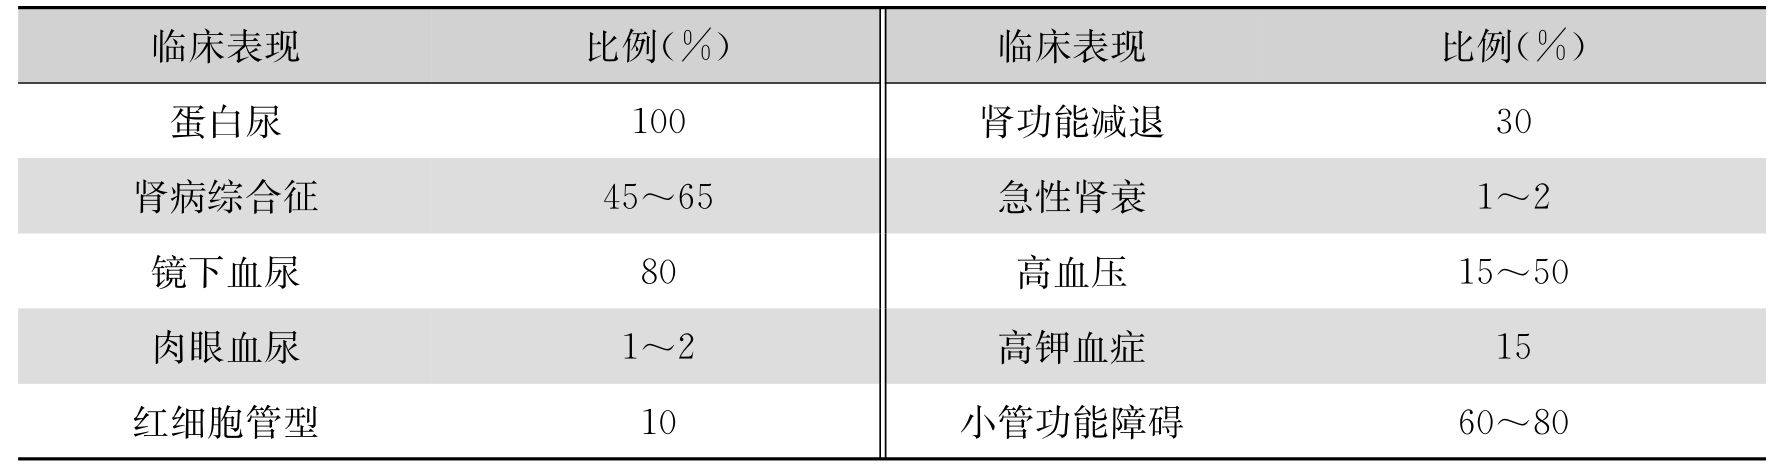
\includegraphics[width=5.91667in,height=1.57292in]{./images/Image00235.jpg}
\end{table}

\begin{longtable}{c}
 \caption{狼疮性肾炎的病理分型(ISN/RPS,2003年)}
 \label{tab37-5}
 \endfirsthead
 \caption[]{狼疮性肾炎的病理分型(ISN/RPS,2003年)}
 \endhead
 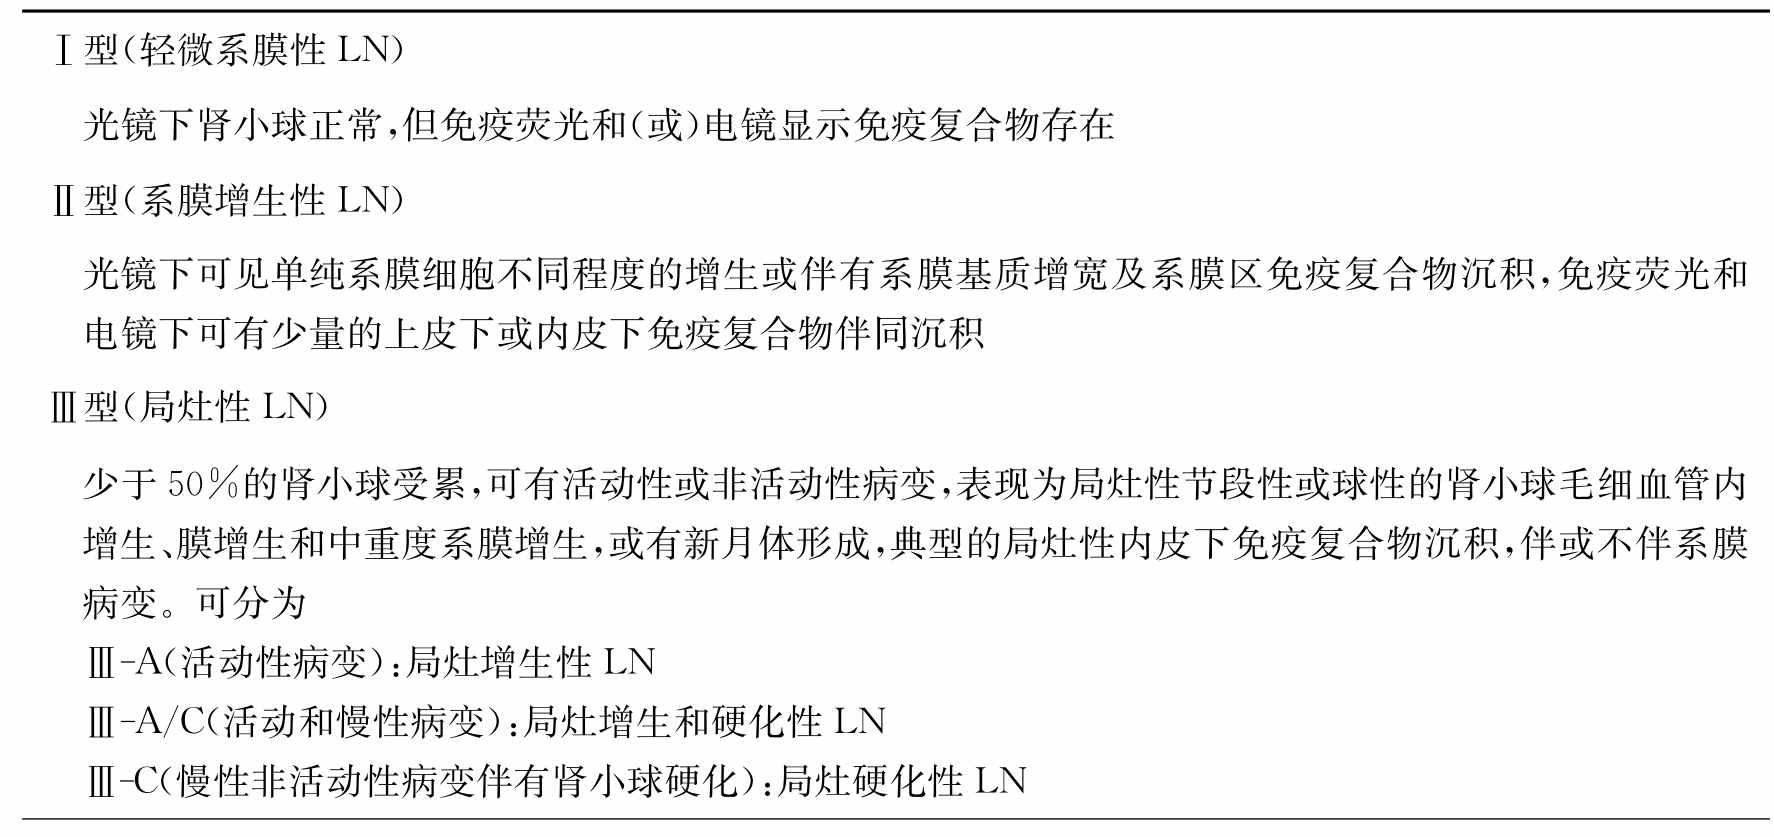
\includegraphics[width=\textwidth,height=\textheight,keepaspectratio]{./images/Image00236.jpg}\\
 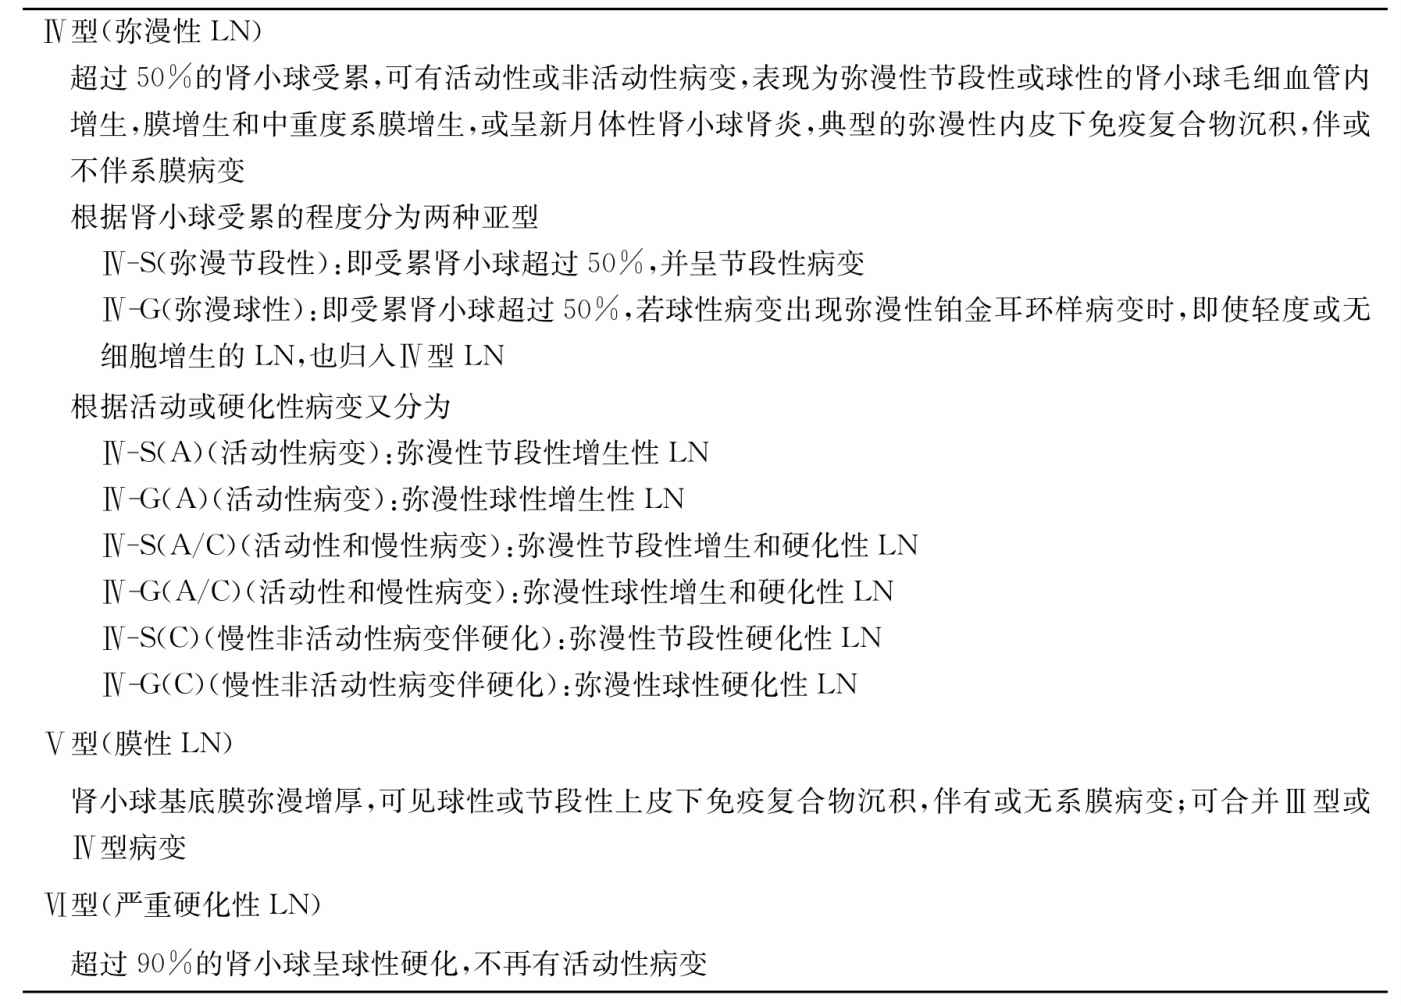
\includegraphics[width=\textwidth,height=\textheight,keepaspectratio]{./images/Image00237.jpg}
 \end{longtable}

国内报道LN占成人继发性肾小球疾病的63.7\%,高发年龄为20~39岁,男女比例为1∶7,临床表现以尿检异常(62.9\%)和肾病综合征(20.42\%)为主。一组25例LN患者中,肾病综合征13例(52\%),其中Ⅳ型7例,Ⅴ型3例,Ⅱ型2例,Ⅲ型1例;肾炎综合征6例(24\%),Ⅳ和Ⅴ型各2例,Ⅱ和Ⅲ型各1例;肾衰竭4例(16\%),均为Ⅳ型。

\subsubsection{(二)紫癜性肾炎(Henoch-Schönlein purpura nephritis,HSPN)}

过敏性紫癜是一种以皮肤、关节、胃肠和肾脏损害为主的多系统疾病。其肾脏损害主要表现为血尿、蛋白尿,多数发生于紫癜出现后2~4周。国内报道肾脏累及率为39.8\%~56.5\%。HSPN好发于10岁以下儿童。病理上以肾小球系膜病变为主,可伴不同程度的新月体形成,免疫病理以IgA颗粒样弥漫性肾小球沉积为特征。临床表现多样,可分为5型:①轻型:表现为轻度无症状性血尿、蛋白尿,无高血压及肾功能损害,病理上多属轻微异常或肾小球局灶、节段性改变,预后好。②急性肾炎型:起病急,似急性肾炎,但只有少数患者同时具有水肿、血尿、高血压三大症状,病理改变多为局灶增生性肾炎或弥漫增生性肾炎。③肾病综合征型:具有典型肾病综合征表现,并以血尿、大量蛋白尿及明显水肿为突出症状,部分病例有肾功能减退,病理上呈弥漫增生性肾炎,伴有不同程度新月体形成,大量新月体(>50\%)者预后差。④急进性肾炎型:起病急骤,早期即出现肾功能减退症状,常伴有心、脑受累。如不及时处理短期内病情恶化,死于肾衰竭,病理上50\%~75\%肾小球有新月体形成。⑤慢性肾炎型:常为上述各型的转归,起病缓慢,肾损害持久存在,伴有慢性肾功能减退,成人多见。病理变化呈弥漫增生性改变,伴有肾小球硬化或新月体形成,预后差。

国内报道HSPN占成人继发性肾小球疾病的11.3\%,多见于13~19岁,男女比例为1.9∶1。有报道160例HSPN患儿,临床表现有单纯性血尿(13.1\%),蛋白尿伴血尿(68.8\%),肾病综合征伴血尿(18.1\%),无表现为急性肾炎综合征、肾病综合征伴肾炎综合征的病例。其中28例病理结果有:弥漫系膜增生性肾炎(43\%),弥漫增生伴新月体和(或)粘连、硬化等局灶性病变(46\%),弥漫性系膜增生伴新月体(比例>75\%)(4\%),膜增生性肾炎(7.1\%)。另报道145例HSPN患儿,临床表现为单纯性血尿(24.1\%),蛋白尿伴或不伴血尿(36.6\%),肾病综合征(24.8\%),急性肾炎(6.2\%),肾病综合征伴肾炎综合征(8.3\%)。

\subsubsection{(三)Goodpasture综合征}

本病是由于肺泡和肾小球毛细血管的基底膜受免疫损害而导致的不同程度咯血和抗GBM抗体性肾炎的临床症候群,罕见但死亡率高。临床特点:①发病以青年居多。②发病前部分患者有流感病毒感染或挥发性烃化物(如汽油)吸入史。③多数患者肺部症状在先,或肺、肾病变同时出现,仅极少数患者首先出现肾病变。④肺部表现:咯血为常见和最早的表现,轻者仅痰带血丝,重者可窒息死亡;常伴咳嗽及气憋,并常出现发热;痰中可见含铁血黄素细胞;胸片可见由肺门向两肺肺野扩散的蝶形阴影,肺尖及肺底很少受累,咯血控制后,此阴影能在1~2周内完全吸收,但反复出血的晚期病例,可呈永久性弥漫网状结节影,提示肺间质纤维化。⑤肾脏表现:病理为新月体性肾炎者临床呈现急进性肾炎,出现蛋白尿(很少呈现大量蛋白尿)、血尿(肉眼或镜下血尿)、水肿及高血压,肾功能急剧恶化,数周至数月即出现少尿或无尿,进入尿毒症期;少数非新月体性肾炎的轻症病例,仅表现为尿异常,肾功能并无变化。⑥贫血很常见,其严重程度常与咯血及肾衰竭程度不平行。

\subsubsection{(四)系统性硬化症肾损害}

系统性硬化症(systemic
sclerosis)是一种以局限性或弥漫性皮肤增厚和纤维化为特征,主要侵犯皮肤及内脏(心、肺、胃肠道和肾)的结缔组织病。好发于生育年龄女性。累及肾脏可表现为蛋白尿,常伴镜下血尿和轻中度高血压及慢性肾功能损害。严重者可发生肾脏危象,易发于老年男性,表现为突发的进展性高血压、急性肾功能不全、微血管内溶血性贫血、消耗性血小板减少伴高肾素血症。

国内报道93例本病患者,肾脏损害发生率为19.4\%,肾衰竭发生率为5.4\%。病理改变主要为肾血管病变。

\subsubsection{(五)干燥综合征(Sjögren's syndrome)肾损害}

是一个主要累及外分泌腺体的慢性炎症性自身免疫病。发病年龄多在40~50岁,也见于儿童,女性多见。

国内报道本病肾脏累及率约30\%~50\%。主要累及远端肾小管,表现为因Ⅰ型肾小管酸中毒而引起的低血钾性肌肉麻痹,严重者出现肾钙化、肾结石及软骨病。近端肾小管损害较少见。小部分患者出现较明显的肾小球损害,临床表现为大量蛋白尿、低白蛋白血症甚至肾功能不全。

已报道3组本病肾损害病例,临床表现均以远端肾小管酸中毒为主(分别为64.3\%,78.9\%和57.1\%),病理表现均以慢性间质性肾炎为主(分别为56.8\%,60.5\%和78.6\%);其中一组病理结果提示肾小球损害并非少见(约60.5\%)。此外本病高γ球蛋白血症的发生率为38.1\%~76.3\%。

\subsubsection{(六)多发性骨髓瘤肾损害}

多发性骨髓瘤(multiple
myeloma,MM)是单克隆浆细胞恶性增生引起的一系列器官功能障碍。多见于中老年人,男性较多。本病肾脏累及率约60\%~90\%,肾损害主要表现在3个方面:①慢性肾小管间质病变:常仅呈现少量蛋白尿(主要为轻链蛋白及肾小管性蛋白尿)及不同程度的肾小管功能损害;②肾小球病变:常出现大量蛋白尿、肾病综合征,若继发肾淀粉样变时,肾功能常进行性衰退;③急性肾衰竭:常突然发生,出现少尿、低比重尿、肾功能急剧恶化,并伴发水、电解质及酸碱平衡紊乱。

国内报道MM肾脏受累者占36.6\%,肾脏受累的表现主要以蛋白尿(68.3\%)和肾功能不全(急性肾衰16.3\%,慢性肾衰35.0\%)为主,血尿、高血压少见,晚期多出现慢性肾功能不全。另报道24例MM肾损害病例,临床上以肾功能不全最为常见(83.3\%),其次为肾病综合征、无症状尿检异常。病理改变以管型肾病最常见(62.0\%),还有慢性间质性肾炎、轻链沉积病、肾小球淀粉样变性和肾小球系膜增生性病变。该资料表明MM肾损害患者具有下列特征:①高血压发生率低;②部分患者在肾衰竭时仍存在大量蛋白尿,但常常不伴有低蛋白血症;③尿沉渣检查常无明显异常;④绝大多数患者合并明显的近端和远端肾小管功能损害;⑤虽然大多数患者已出现肾功能不全,但B超显示双肾并无明显缩小。

\subsubsection{(七)肝病相关性肾小球肾炎}

肝病患者常合并有尿检异常或肾功能下降,而在肝病并发的肾损害中以肾小球疾病最为多见。

\paragraph{1.HBV相关性肾小球肾炎(HBV associated glomerulonephritis,HBV-GN)}

男性多见,多见于儿童及青少年。肾脏病理改变依次为膜性肾病,膜增生性肾炎,系膜增生性肾炎,微小病变,局灶性肾小球硬化和IgA肾病样改变。

膜性肾病是最常见的病理类型,临床呈一良性过程,多表现为肾病综合征;部分表现为单纯性血尿或蛋白尿;1/4患者合并肾功能不全;1/3伴有高血压。系膜毛细血管性肾炎以肾病综合征伴镜下血尿多见,半数患者伴有高血压,1/3伴发肾功能不全。

国内报道62例HBV-GN病例,少儿发病率最高(67.7\%),临床上大多数无症状,常常是体检时发现尿常规异常、血乙肝抗原阳性行肾活检而发现;有症状者主要表现为肾病综合征、镜下血尿,部分可有转氨酶升高。青壮年症状较少儿重,多表现为肾病综合征、镜下血尿和(或)大量蛋白尿。中老年人发病率相对较低(9.7\%)。病理类型上,少儿以膜性肾病(45.2\%)最多见,其次是膜增生性肾炎、系膜增生性肾炎、局灶性节段性肾小球硬化;青壮年与中老年人则以膜增生性肾炎(分别为35.7\%和33.3\%)为最常见,其次是膜性肾病、系膜增生性肾炎、局灶性节段性肾小球硬化、IgA肾病样改变。

\paragraph{2.HCV相关性肾小球肾炎}

肾脏病理改变最常见为膜增生性肾炎,其次为膜性病变,IgA肾病样改变,感染后肾炎,局灶节段性肾炎,此外,尚有个别病例表现为免疫管状肾病、肾脏小血管炎、小叶间动脉坏死性炎症。

膜增生性肾炎临床表现为肾病性或非肾病性蛋白尿、镜下血尿、轻中度肾功能不全;如血清HCV抗体、HCV-RNA阳性、转氨酶升高、RF阳性及低补体血症均支持HCV相关的膜增生性肾炎,50\%~70\%患者伴有高冷球蛋白血症。膜性肾病多表现为肾病综合征,少数为单纯性蛋白尿或非肾病性蛋白尿,补体水平正常,肝功能正常,RF阴性,可伴有冷球蛋白血症。

\paragraph{3.肝硬化相关性肾小球肾炎}

约10\%的肝硬化成人患者合并镜下血尿和(或)中等量蛋白尿。肾脏病理类型主要包括继发性IgA肾病、肝性肾小球硬化,少数患者呈膜性病变、新月体性病变、系膜毛细血管性病变及毛细血管内增生性病变。

肝硬化继发性IgA肾病以酒精性肝硬化尤为多见,一般起病隐匿,进展缓慢,呈良性过程,表现为镜下血尿、少量蛋白尿或中度肾功能受损。

\subsubsection{(八)糖尿病肾病(diabetic nephropathy,DN)}

DN是糖尿病代谢异常引发的肾小球硬化症,是糖尿病的常见并发症,也是糖尿病患者的主要死亡原因之一。据统计,1型糖尿病肾病的发生率为30\%~40\%,2型则为20\%~60\%。1型糖尿病通常在确诊后15~20年发生糖尿病肾病,而2型则较1型短5~10年。国内报道2型糖尿病肾病的患病率为9.73\%,终末期肾病的患病率为5.47\%。另报道老年人继发性肾小球病以DN最常见(14.2\%)。

DN的基本病变是肾小球基底膜增厚和系膜基质的增生,包括弥漫型肾小球硬化和结节型肾小球硬化两种。临床特点:①1型DN自然病程较清晰,可参照Mogensen分期分为5期:Ⅰ、Ⅱ期仅有肾小球滤过率升高,肾脏体积增大,无其他临床异常;Ⅲ期为微量白蛋白尿期,其标志为尿白蛋白排泄率(UAER)持续位于20~200μg/min之间;若UAER>200μg/min或尿蛋白>0.5g/d,则进入Ⅳ期,临床上逐步加重,表现为肾病综合征、高血压、肾功能缓慢恶化;Ⅴ期为终末期肾病(ESRD),需要透析等替代治疗。临床上典型者约每5年进展1期。②2型DN与1型有如下不同:开始时,肾小球高滤过发生率较1型少见(50\%vs.90\%);高血压出现早、发生率高,在微量白蛋白尿期即有约60\%的患者合并高血压(1型约为20\%),进入肾病综合征后上升为80\%~90\%(1型约为60\%);病程经过多样;多数患者经由微量白蛋白尿进入肾病综合征直至ESRD,但有10\%~15\%的患者在诊断糖尿病同时出现大量蛋白尿,甚至肾功能不全。因此,临床上倾向于将2型DN分为隐性DN(早期)、显性DN及终末期DN,分别相当于1型中的Ⅲ、Ⅳ、Ⅴ期。

\subsubsection{(九)高尿酸血症肾病(hyperuricemic nephropathy)}

高尿酸血症肾病是指由于嘌呤代谢紊乱使血尿酸生成过多或由于肾脏排泄尿酸减少,尿酸盐在血中呈过饱和状态时沉积于肾脏而引起的肾脏病变。其主要表现有:①慢性高尿酸血症肾病(痛风性肾病):由于尿酸盐沉积肾小管间质所致,早期常无症状,肾小管功能,尤其是浓缩功能减退常为最早表现,尿检异常出现较晚且轻微,仅见轻度蛋白尿(以小分子蛋白尿为主)及少量红细胞,晚期肾小球滤过率下降,最终发展至慢性肾衰竭。②急性高尿酸血症肾病:常见于血尿酸急剧增高的患者,尿中尿酸排出增多,尿酸盐在集合管、肾盂及输尿管沉积,出现少尿以至无尿,尿中可见红细胞及尿酸结晶,起病突然,迅速发展为氮质血症,甚至肾衰竭。③尿酸结石。

国内报道痛风性肾病占原发性痛风的60\%,痛风性肾病患者中,以50岁以上的男性多见(79\%),81\%伴有肾功能减退,以肾小管功能损害更显著,22.6\%有泌尿系结石。另报道216例痛风患者,21.8\%合并有泌尿系透光结石,12.9\%发生肾功能不全。

\subsubsection{(十)自身免疫性甲状腺疾病相关性肾病}

自身免疫性甲状腺疾病,包括Graves病、慢性淋巴细胞性甲状腺炎和原发性甲状腺功能减退症,是临床常见的一类疾病,当患者出现肾损害时称为自身免疫性甲状腺疾病相关性肾病。本病均有蛋白尿,可为轻微蛋白尿,少数呈肾病综合征。

国内报道16例本病患者,均出现不同程度蛋白尿,其中5例(31.3\%)呈肾病综合征,10例(62.5\%)有不同程度的镜下血尿。其病理改变以非IgA系膜增生性肾炎(37.5\%)最常见,其次为膜性肾病(25\%)和局灶节段性肾小球硬化(25\%),此外还有微小病变和IgA肾病样改变。

\subsubsection{(十一)肾淀粉样变性病(renal amyloidosis)}

淀粉样变性病是一种以淀粉样物质沉积于心脏、肾脏、消化道等脏器所引起的疾病,国内报道肾脏累及率达75\%。淀粉样物质沉积于肾脏引起的肾病变称为肾淀粉样变性病。多见于50岁以上男性。临床上以肾病综合征为主要表现,晚期可导致肾衰竭。本病为老年继发性肾病综合征的常见病因。根据临床表现可分为4期:①临床前期:无任何临床表现,仅肾活检可作出诊断;②蛋白尿期:蛋白尿为常见的早期表现,可出现蛋白尿伴镜下血尿,但细胞管型少见,肉眼血尿罕见,可伴轻至中度高血压;③肾病综合征期:一旦出现肾病综合征,病情进展迅速,预后差;④尿毒症期:出现肾功能进行性减退,除肾小球受累外,肾小管间质均可受累,出现多尿、低比重尿、甚至尿崩症等。肾病理学特点为刚果红染色阳性和(或)电镜下可见8~10nm不分支的纤维丝样物质。

国内报道9例本病患者中,6例呈肾病综合征,其中伴肾衰竭2例,大量蛋白尿伴镜下血尿1例,单纯性蛋白尿2例;血肌酐增高6例。肾活检示肾小球或系膜区毛细血管壁刚果红染色阳性9例,肾小管上皮呈阳性4例,7例电镜下见毛细血管壁及系膜区细纤维管状结构沉积。另报道25例本病患者,临床表现有蛋白尿(100\%,其中48\%为肾病综合征)、镜下血尿(12\%)和肾功能不全(40\%)。

\subsubsection{(十二)高血压肾病}

原发性高血压发生5~10年后常伴有靶器官损害,肾脏是最易受累的器官之一。一旦发生肾损害,则称为高血压肾病。临床上常将高血压肾病分为良性小动脉性肾硬化和恶性小动脉性肾硬化。

良性小动脉性肾硬化是良性高血压发展的结果。其主要病变为入球小动脉玻璃样变,小叶间动脉及弓状动脉肌内膜肥厚;随着血管壁增厚,管腔狭窄发展,导致肾小球和肾小管缺血性病变,最终导致肾小球萎缩硬化,肾小管萎缩、间质纤维化。临床特点:①发病年龄一般在40~60岁,特别好发于合并糖尿病或长期高血压控制不良者。②轻度肾损害时,尿微量白蛋白排出增加,尿沉渣红细胞计数增加,可见畸形红细胞,尿β2-微球蛋白及N-乙酰\textsuperscript{-}
β\textsuperscript{-}
葡萄糖苷酶(NAG)排出增加,此时若血压控制良好上述变化可减轻。中度肾损害时,首发症状是夜尿增多,继之出现蛋白尿,一般表现为轻至中度蛋白尿(24小时尿蛋白定量一般不超过1.5~2.0g),很少出现大量蛋白尿,有些可合并有镜下血尿,蛋白尿排出量可随血压升高而增加,随血压控制而减少。重度肾损害,当肌酐清除率降至50ml/min时,患者可在发热、外伤、感染、药物中毒等应激情况下出现氮质血症,且不易恢复;但肾性贫血相对比较轻,并易发生高尿酸血症,少数发展成尿毒症。③常合并其他脏器损害,如高血压性左心室肥厚,脑动脉硬化引起的脑血管意外和视网膜动脉硬化等。

恶性小动脉性肾硬化是由恶性高血压所致的严重肾损害。主要病变是入球小动脉纤维素样坏死和肾叶间动脉纤维样动脉内膜炎。临床特点:①大多数发病前有良性高血压史,平均发病年龄为40~50岁。②恶性高血压发病急骤,表现为血压明显升高,舒张压一般都超过120~130mmHg,首发症状是头痛、头晕,伴视力模糊、视乳头水肿、体重下降、呼吸困难、恶心呕吐、疲劳、上腹痛、多尿、夜尿增多和肉眼血尿,严重时出现左心衰竭、昏迷、抽搐甚至脑出血。③恶性小动脉性肾硬化常首先表现为突发蛋白尿,24小时尿蛋白定量<2g、2~4g、>4g者各占1/3,伴无痛性肉眼血尿(20\%)或镜下血尿(50\%),甚至出现红细胞管型;大多数患者可出现白细胞尿;肾功能急剧恶化,BUN及Scr进行性升高,迅速进展至肾衰竭;肾脏大小正常或增大或轻度缩小。

\subsubsection{(十三)ANCA相关性肾炎(ANCA associated nephritis)}

原发性小血管炎(primary small vessel
vasculitis,PSV)包括Wegener肉芽肿、显微镜下型多血管炎和变应性肉芽肿性血管炎,由于其与抗中性粒细胞胞浆抗体(ANCA)密切相关,也称ANCA相关性小血管炎。本病好发于中、老年男性。

肾脏最易受累,国内报道肾脏累及率为94\%~96.4\%。早期表现有血尿,其中1/3为肉眼血尿;蛋白尿很常见,但很少出现肾病性蛋白尿;多数呈急进性肾炎综合征;高血压不多见或较轻;肾功能常进行性损伤,如能及时合理治疗,有些病例可完全恢复。肾脏病变以肾小球坏死性新月体病变为特征。光镜下可见:局灶节段性肾小球毛细血管袢坏死,新月体形成;髓质肾小管周围毛细血管炎;肾小管间质炎症细胞浸润,有时形成肉芽肿。免疫病理和电镜检查未发现免疫复合物。

国内报道34例本病患者,17例以急性肾衰竭起病,其余多表现为肾炎综合征,3例就诊时已为ESRD。急性肾衰竭者肾脏病理多为局灶节段性纤维素样坏死和新月体肾炎;而肾炎综合征者病理也可为局灶节段性纤维素样坏死和新月体肾炎,而且病理上病变可多种多样,也可以新鲜病变(如纤维素样坏死)和陈旧病变(如肾小球硬化)并存。另报道54例本病患者,临床表现为血尿(100\%,多为镜下血尿),蛋白尿(88.9\%,其中10.4\%为肾病综合征)和血肌酐增高(75.9\%,其中50\%为急性肾衰竭)。病理表现为新月体性肾炎(11/20),局灶坏死性肾小球肾炎(5/20),轻度系膜增生性肾小球肾炎(4/20)和肉芽肿性小血管炎(3/20)。

\subsubsection{(十四)类风湿关节炎(rheumatoid arthritis,RA)}

类风湿关节炎是一类临床常见的慢性炎症性自身免疫性结缔组织疾病,各年龄均可发病,多见于40~60岁。RA临床表现多样,可累及多系统、多脏器,其典型表现为全身任何关节的对称性多关节炎,以双手腕关节、掌指关节和近端指间关节最为常见,可伴有轻中度发热、贫血、类风湿性小结节、心包炎、肾炎、系统性血管炎及淋巴结肿大等关节外表现。RA最突出的病理表现为关节滑膜炎,引起关节畸形。RA的肾脏损害较为常见,以尿检异常为准,肾脏损害的发生率为20\%~55\%,肾活检资料提示肾脏病变发生率可达100\%。RA的肾脏损害主要分为3类:①原发性,包括多种,肾小球肾炎和肾小管间质性肾炎;②肾脏淀粉样变性;③继发性,多与治疗RA药物有关。肾脏损害的临床表现主要为单纯蛋白尿、单纯镜下或肉眼血尿、蛋白尿和血尿并存,尿比重及pH异常,甚至出现肾病综合征、慢性肾衰竭。

国内报道42例RA合并肾损害患者均存在蛋白尿,64.3\%伴血尿,50\%伴高血压,33.3\%血肌酐升高。病理改变以系膜增生性病变伴IgA沉积(28.6\%)和不伴IgA沉积(26.2\%)最常见,其次为膜性病变(23.8\%),节段坏死性肾炎(16.7\%),膜增生性肾炎(4.7\%)。另有报道20例RA合并肾损害患者,慢性肾炎是最常见表现(8例),其次为肾病综合征(4例),而系膜增生性肾炎、膜性肾病是RA并发肾炎的常见病理类型。

\subsubsection{(十五)感染性心内膜炎(infectious endocarditis,IE)}

感染性心内膜炎指由细菌、真菌或其他病原体(如病毒、立克次体、衣原体、螺旋体等)直接感染而引起的心瓣膜或心室壁内膜的炎症并伴赘生物形成,常多发于原有心瓣膜疾病、先天性心血管畸形、长时间经静脉治疗、静脉注射药物成瘾、由药物或疾病引起免疫抑制及人工瓣膜置换术后。IE典型临床表现包括发热、心脏杂音、贫血、栓塞、皮肤损害、脾大和血培养阳性等,但均非特异性表现。IE引起肾损害的临床及病理表现包括以下4个方面:①肾局灶梗死:为最常见肾损害,多由心瓣膜上赘生物脱落,引起肾脏小动脉栓塞及肾脏楔形坏死。临床表现主要为腰部疼痛,肉眼血尿,肾功能急剧恶化。出现肾梗死比较局限,一般肾活检均难以取到梗死灶。②肾小球肾炎:病情较轻者通常为局灶节段性肾小球肾炎,病理改变主要是节段内皮细胞、系膜细胞增生,少量中性粒细胞和单核细胞浸润,基膜正常。临床表现为持续性镜下血尿、白细胞尿、少至中等量蛋白尿,肾功能正常。病情严重者表现为急进性肾炎,病理改变为弥漫增生性肾炎,大量中性粒细胞和单核细胞浸润或伴袢坏死,基膜双轨,同时存在细胞性或纤维细胞性新月体,肾小管间质病变重。临床表现为大量蛋白尿、镜下血尿,伴肾功能不全,但高血压发生率不高,肉眼血尿少见。③急性间质性肾炎和急性肾小管坏死:心衰或败血症休克可导致急性肾小管坏死的出现。同时,由于肾小球病变相伴的小管间质病变以及抗生素的广泛应用,急性间质性肾炎也较为常见。④ANCA相关的肾血管炎:较为少见,血清C-ANCA或P-ANCA阳性。

国内报道155例IE患者,其中伴肾脏损害137例(88.4\%),表现包括无症状血尿和(或)蛋白尿(71.0\%)、急性肾炎综合征(6.5\%)、肾病综合征(2.6\%)、急进性肾炎综合征(1.3\%)、肾栓塞(1.3\%)、单纯白细胞尿(3.2\%)、非IE直接所致肾损害(2.6\%)。其中肾活检4例,分别为弥漫增生性肾小球肾炎、膜性肾病Ⅱ期、膜增生性肾小球肾炎及Ⅱ型新月体肾炎各1例。另报道75例IE患者,其中伴肾脏损害59例,表现为血尿和(或)蛋白尿(86.4\%),急性肾炎综合征(4.8\%),肾病综合征(1.7\%),急进性肾炎(3.4\%),肾栓塞(3.4\%)。另报道2例静脉吸毒继发感染性心内膜炎合并肾损害,主要表现为发热、水肿、蛋白尿(3+-4+)、血尿;肾脏病理示:重度系膜增生性肾小球肾炎,急性间质性肾炎。

\subsubsection{(十六)POEMS综合征}

POEMS综合征是少见的与浆细胞有关的以多系统损害为特征的临床综合征,具有多发性周围神经病变、肝、脾等脏器肿大、内分泌病变、单克隆免疫球蛋白和皮肤改变(polyneuropathy,organomegaly,endocrinopathy,monoclonal
gammopathy and skin
changes,POEMS)五大特点,POEMS由上述症状的英文首字母组合而成。本病首发症状出现顺序不一,表现复杂多变,但神经系统症状与浆细胞病一般都存在,当有以上五项主征中三项以上又排除了其他慢性周围神经病时即可确诊。POEMS综合征相关性肾病最常见表现为轻中度蛋白尿、水肿、镜下血尿、管型;急性肾衰竭伴恶心、呕吐,慢性肾功能不全以及需行替代治疗的终末期肾衰竭也较常见。肾脏的病理改变以肾小球为主,早期为三类病理变化特征:即肾小球膜增生样病变、微血管病变和系膜溶解性病变,晚期病变逐渐进展发生单侧或双侧肾脏变小及非炎性纤维化动脉内膜炎。

国内报道12例POEMS综合征患者,肾脏损害表现主要为水肿11例(91.7\%),少量蛋白尿8例(66.7\%),镜下血尿1例(8.3\%),血清肌酐升高6例(50\%),尿酸升高11例(91.7\%)。其中4例行肾活检,病理特点为:①肾小球系膜病变明显,以系膜区增宽、系膜细胞及基质增生、系膜溶解改变为主;②肾小球内皮细胞病变突出;③未见免疫复合物沉积。另有报道12例POEMS综合征患者,肾脏受累者占25\%,最常见的表现为轻度至中度蛋白尿、水肿、镜下血尿;病理呈现膜增生性肾小球肾炎样病变,个别肾小球见λ轻链沉积。

\subsubsection{(十七)IgG\textsubscript{4} 相关系统性疾病(IgG\textsubscript{4}}
-related systemic disease,IgG4-RSD)

IgG\textsubscript{4} 相关系统性疾病是新近被提出的与IgG\textsubscript{4}
淋巴细胞密切相关的慢性、系统性疾病,又称为IgG\textsubscript{4}
阳性多器官淋巴细胞增生综合征。常累及全身多部位腺体(如胰腺、泪腺、唾液腺)及全身多部位淋巴结、腹膜后组织、肾脏、垂体等,临床特点为单一或多个器官、组织肿胀增大,类似肿瘤;病灶组织浆细胞浸润伴IgG\textsubscript{4}
高表达、纤维化;血清IgG\textsubscript{4}
水平明显升高;对免疫抑制治疗反应良好。IgG\textsubscript{4}
-RSD临床表现主要有以下几个方面:①自身免疫性胰腺炎;②IgG\textsubscript{4}
相关淋巴结病;③IgG\textsubscript{4}
相关性桥本甲状腺炎;④米库利奇病(Mikulicz
disease);⑤其他器官受累:如垂体、腹膜后组织、肺部等。IgG\textsubscript{4}
-RSD引起肾脏受累主要包括以下2方面:①IgG\textsubscript{4}
-RSD累及肾脏:引起IgG\textsubscript{4}
相关的间质性肾炎、IgG\textsubscript{4}
相关膜性肾病、肾炎性假瘤,常表现为急性或慢性肾功能不全及蛋白尿(大部分尿蛋白定量<1g/24h,少数尿蛋白定量>1g/24h者可能合并肾小球损害);②IgG\textsubscript{4}
-RSD相关的腹膜后纤维化、前列腺炎或输尿管炎性改变所造成肾后性梗阻性肾病(伴或不伴肾脏间质损害)。多表现为非特异性的畏寒、发热、疲劳和体重减轻等症状,背部疼痛、侧腹或下腹部疼痛最常见。腹膜后纤维化包块可压迫输尿管致输尿管梗阻和肾积水。肾脏病理常表现为小管间质性肾炎(tubulointerstitial
nephritis,TIN),也可同时伴有肾小球病变(以膜性肾病多见)。

国内报道6例IgG\textsubscript{4}
-RSD泌尿系统损害患者,男女比例为4∶2,除肾脏、输尿管受累外,均同时存在泌尿系统外的多器官受累。肾脏损伤表现主要为肾功能异常、水肿和腹痛。所有患者均存在肾小管源性蛋白尿,无肉眼血尿,5例患者血清Cr显著升高。肾脏病理示弥漫纤维化伴肾间质大量淋巴细胞、浆细胞浸润的间质性肾炎表现,伴淋巴细胞、浆细胞IgG\textsubscript{4}
免疫组化染色阳性。另有报道2例IgG\textsubscript{4}
相关小管间质性肾炎,肾脏受累表现主要为少量蛋白尿、偶见镜下血尿伴肾功能损伤。肾脏病理特点为肾间质中大量IgG\textsubscript{4}
阳性浆细胞浸润、间质纤维化。

\subsubsection{(十八)轻链沉积病(light chain deposition disease,LCDD)}

轻链沉积病是一种少见的由异常浆细胞产生过多,引起单克隆免疫球蛋白轻链的大量产生并沉积于全身组织而导致的一种系统性疾病,多发于45岁以上中老年人。约60\%的LCDD继发于淋巴细胞增生性病变,如多发性骨髓瘤、淋巴瘤、华氏巨球蛋白血症等;其余40\%病例缺乏浆细胞病的证据。肾脏为其最常见的受累器官。以不同程度的蛋白尿和急性肾衰或进展型慢性肾衰最为常见,多表现为肾病综合征,部分可伴高血压及镜下血尿,有些可出现肾小管间质病变。肾脏典型病理改变为系膜结节状硬化性肾小球病,结节常为多个,肾小管基底膜增厚、皱缩及分层,其外侧可见均质粉染的蛋白物质沉积,刚果红染色阴性,免疫荧光检查发现单种轻链蛋白弥漫、线性沉积于肾小球、肾小管基底膜、结节内及各级血管壁上,具有决定性诊断意义。

国内报道26例本病患者中,急性肾衰3例,慢性肾衰17例,肾病综合征17例,肾脏病理改变以系膜结节样病变多见(53.8\%),中至重度小管间质慢性化病变为该组病例较特征性病变(92.3\%)。另有报道12例轻链蛋白沉积肾损害病例,其中6例表现为肾衰竭,5例表现为肾病综合征,病理均显示λ轻链蛋白主要沉积在肾小球系膜区、基底膜、肾小管基底膜及小动脉壁。

\subsubsection{(十九)重链沉积病(heavy chain deposition disease,HCDD)}

重链沉积病是一种罕见的、病因不明的淋巴浆细胞增生性疾病,以单克隆免疫球蛋白重链沉积于组织器官并造成功能障碍为特征。依据重链抗原的不同,该病可分为三种:γ(IgG)、α(IgA)和μ(IgM),其中γ重链可分为γ1、γ2、γ3、γ4等亚型。该病多发病年龄偏大,无明显性别差异;起病常缓慢,临床表现为贫血,反复感染,肝、脾、淋巴结肿大,常有腭部、腭垂水肿,伴Waldeyer扁桃体环等,罕见累及皮肤及甲状腺的病例。目前,本病肾脏累及率几乎100\%,并通过肾活检确诊。肾脏受累主要表现为肾病综合征、蛋白尿、水肿、镜下血尿、高血压和肾功能不全,多数快速恶化进展为终末期肾衰竭。多数可在血清、尿液或骨髓涂片检测到单克隆免疫球蛋白,尿中无轻链蛋白。肾活检病理多以系膜区增宽,基质增多,肾小球弥漫结节性硬化为特征表现,结节PAS染色阳性,细胞数轻度增多,可有新月体形成;肾小管可见不同程度萎缩、基膜增厚,并有PAS阳性、刚果红阴性的物质沿基膜外缘线样沉积。动脉、小动脉、管周毛细血管基膜均可以有相同性质的沉积物,小动脉壁玻璃样变和内膜纤维化。单克隆免疫荧光重链染色是确定HCDD的重要手段。

国内报道3例本病肾损害病例,临床表现为:大量蛋白尿(>5g/L)、镜下血尿,高血压伴肾功能不全及贫血。肾活检为弥漫肾小球结节样病变,免疫荧光染色示IgG沿肾小球毛细血管袢及肾小管基膜呈线样沉积,轻链染色阴性。

\subsubsection{(二十)人类免疫缺陷病毒感染相关性肾病(human immunodeficiency}
virus-associated nephropathy,HIVAN)

人类免疫缺陷病毒感染相关性肾病是由是人类免疫缺陷病毒(human
immunodeficiency
virus,HIV)感染导致的一种肾脏疾病。HIVAN是HIV感染患者肾脏损伤最常见的类型,可出现在HIV感染的任何阶段,以大量蛋白尿、快速进展性肾衰竭为主要临床表现,90\%患者蛋白尿可至肾病综合征水平,而且常早期出现,甚至个别高达20g/24h;多数患者伴有镜下血尿,可不伴有明显高血压、水肿、低蛋白血症及高脂血症。肾脏病理改变包括塌陷型局灶节段性肾小球硬化,足细胞增殖肥大,肾小管的空泡样改变-微囊性扩张、间质纤维化和间质炎性反应。电镜下可见肾小球内皮细胞和(或)肾小管上皮细胞内HIV病毒颗粒或细胞核内及胞质内管状网状包涵体。

国内报道2例HIV合并肾脏疾病患者,表现为大量蛋白尿(肾病综合征),肾功能不全,伴持续镜下血尿和高血压,其中1例肾活检示轻度局灶节段性肾小球硬化,肾小管空泡变性,肾间质淋巴细胞浸润。

\subsubsection{(二十一)肿瘤相关性肾病}

大多数恶性肿瘤包括:血液系统肿瘤,如白血病、淋巴瘤、多发性骨髓瘤等;实体肿瘤,如肺癌、胃肠道肿瘤、食管癌、乳腺癌等均可引起肾损害。多见于50岁以上男性。肾脏受累的临床症状多无特异性,且易被肿瘤症状所掩盖,典型的肾病综合征是最常见的肿瘤相关性肾病临床表现,肾小球性蛋白尿,少数可有血尿、高血压,肾功能可有不同程度的损伤,甚至终末期肾衰竭。肾脏病理类型主要有:膜性肾病、微小病变肾病和膜增生性肾炎;少见有局灶节段性硬化、新月体性肾炎等。多数患者肿瘤发现的时间常早于或同时于大量蛋白尿的出现,但少数患者恶性肿瘤发生在膜性肾病、微小病变肾病和膜增生性肾炎之后,甚至数十年之久。这类患者当肿瘤切除或化疗、放疗后,肾损害的症状可得到缓解。

国内报道15例肿瘤合并肾损害患者,其中肺癌最多(3例),表现为肾病综合征4例,慢性肾小球肾炎4例,慢性肾衰竭7例,该资料提示肾脏损害多为中老年肿瘤患者。另有报道8例实体肿瘤相关肾小球病患者,肺癌和结肠癌居多,各占3例,临床表现为从无症状性蛋白尿至肾病综合征,3/8合并镜下血尿,4/8有不同程度肾功能损伤,4/8存在与肾功能不相符的贫血,2/8存在不能用蛋白尿解释的低白蛋白血症,2/8出现IgG升高。4/8患者经肿瘤治疗后蛋白尿减少或肾功能改善。其中2例行肾活检分别示微小病变肾病和膜性肾病。该资料表明实体肿瘤可以肾小球损伤为首发症状。

\subsubsection{(二十二)肥胖相关性肾病(obesity-related glomerulopathy,ORG)}

肥胖相关性肾病是指由肥胖引起的肾脏损害,根据病理特征的不同,分为肥胖相关性肾小球肥大症(obesity-associated
glomerulomegaly,OB-GM)和肥胖相关性局灶节段性肾小球硬化(obesity-associated
focal and segmental
glomerulosclerosis,OB-FSGS)。本病多见于成年肥胖患者,老年及儿童肥胖者也可发生,男性多于女性。本病突出临床表现主要为肥胖和蛋白尿,早期仅为微量白蛋白尿,随病程逐渐增多至少到中等量蛋白尿,直到出现肾病范围的大量蛋白尿,但很少出现低白蛋白血症、水肿及肾病综合征;另有高脂血症、高血压等表现,一般无肉眼血尿,镜下血尿比例较低(约1/5患者);近半数患者存在肾小管功能异常,部分患者伴肾功能不全,可缓慢进展至终末期肾衰竭,需行肾脏替代治疗。肾脏病理特征为单纯性肾小球肥大和局灶节段性肾小球硬化伴肾小球肥大。前者仅表现肾小球体积增大,系膜区增宽、系膜细胞增生及基质增加可不明显,部分肾小球血管袢内皮细胞可见肿胀,甚至泡沫样变性,免疫荧光检查为阴性。后者与经典的FSGS相似,可见肾小球局灶、节段性硬化,以脐部、顶部较多见,未硬化的肾小球体积可增大,肾小管肥大,部分可见小灶性小管萎缩和纤维化肾间质炎症细胞浸润,免疫荧光可见病变肾小球受累区域IgM和C3沉积,电镜下可见不同程度的足细胞肥大、足细胞密度减少、足突融合。

国内报道15例ORG患者,80\%患者出现非肾病范围的以中等分子量为主的蛋白尿,33\%患者有镜下血尿,无贫血。血清三酰甘油升高者较胆固醇升高者多(分别为53.3\%和40\%),46.7\%的患者血尿酸升高,高胰岛素血症常见(3/5例),此外5例患者谷丙转氨酶升高(33.3\%),54.5\%的患者肝脏B超检查存在脂肪肝。病理改变为肾小球体积增大,伴/不伴节段硬化,其他形态学改变如透明变性、内皮性泡沫细胞及顶部病变等也见于ORG患者。电镜观察足突融合、微绒毛化不广泛,但早期即存在基膜增厚。另报道90例ORG患者,有如下特点:①ORG占所有肾活检的比例为0.89\%,以青年人为主,男性患者占67\%;②100\%为腹型肥胖,其中,轻度肥胖(BMI
28.0~<30kg/m\textsuperscript{2} )、中度肥胖(BMI
30~<35kg/m\textsuperscript{2}
)和重度肥胖(BMI≥35kg/m\textsuperscript{2}
)的患者分别占49\%、37\%和14\%;③平均尿蛋白为(1.48±1.2)g/24h,少量蛋白尿者(0.4~1.0g/24h)占51.1\%,大量蛋白尿者(>3.5g/24h)占10\%,表现为典型肾病综合征者仅2例(2.22\%);④42.2\%患者有肾小球高滤过,6.67\%有肾功能减退;⑤同时合并多种代谢紊乱,88.1\%有胰岛素抵抗,75.0\%有脂代谢异常及63.1\%有高血压;⑥病理特征是肾小球体积增大,70\%合并局灶节段性肾小球硬化(FSGS),并以“经典型”节段硬化为主;⑦随着BMI的增加,ORG患者的蛋白尿水平、肾小球滤过功能及足突宽度显著增加。

\subsubsection{(二十三)多发性肌炎与皮肌炎(polymyositis,PM,dermatomyositis,DM)}

多发性肌炎与皮肌炎是一种病因及发病机制尚不明确,以累及皮肤及横纹肌为主要病变的非化脓性自身免疫性疾病。其临床特征主要为肢体近端肌、颈肌及咽肌等肌组织出现炎症、变性改变,导致对称性肌无力和一定程度的肌萎缩,并可累及多个系统和器官,可能同时伴发肿瘤。若肌炎伴有特征性皮疹则为皮肌炎。女性多见,发病年龄呈现5~14岁和45~60岁两大高峰。该病合并肾脏损害可以表现为肾病综合征,可有镜下血尿、蛋白尿、管型尿,轻中度高血压,肾功能损害多较轻,但也可发生血肌红蛋白升高,阻塞肾小管导致急性肾衰竭。

国内报道146例PM和DM患者,其中30例患者(20.5\%)出现不同程度的肾脏损害,表现为单纯血尿者10例(33.33\%),单纯蛋白尿6例(20.00\%),蛋白尿合并血尿13例(43.33\%),高血压7例(23.33\%),水肿3例。10例单纯血尿患者中,镜下血尿>+++者7例;11例接受24h尿蛋白定量检测患者中,尿蛋白<1g/d者7例;4例行肾活检示局灶节段性肾小球硬化2例,肾小球轻微病变和狼疮性肾炎各1例。

\protect\hypertarget{text00293.html}{}{}

\subsection{三、肾小管间质疾病}

\subsubsection{(一)肾盂肾炎(pyelonephritis)}

急性肾盂肾炎是由于细菌侵入肾脏,引起急性间质性肾炎和肾小管损害。急性肾盂肾炎时离心尿行尿蛋白定性检查常阴性,或感染控制后,随着白细胞尿的阴转尿蛋白消失。一般为上行性感染,最常见的致病菌为大肠杆菌。临床表现为:①尿路局部症状,包括膀胱刺激症状(尿频、尿急、尿痛),腰部或肋脊角压痛和叩痛,偶可伴腹部疼痛;②全身感染症状,如寒战、发热等。若无复杂因素存在,一般极少发展为慢性肾盂肾炎和肾衰竭。

慢性肾盂肾炎多发生于尿路解剖或功能上有异常情况。病理改变除慢性间质性肾炎外,还必须有肾盂和肾盏的炎症、变形和纤维化或肾盏内有脓液。临床表现为:①尿路感染症状,但症状不典型或仅为无症状细菌尿;②慢性肾小管间质损害表现,肾小管功能损害往往比肾小球功能损害更为突出而不成比例。慢性肾盂肾炎一旦出现持续性蛋白尿提示肾小球出现进行性损害,蛋白尿是本病预后不良的指标之一。

\subsubsection{(二)间质性肾炎}

\paragraph{1.急性间质性肾炎(acute interstitial nephritis,AIN)}

AIN是由多种病因引起,起病急骤,以肾间质水肿和炎症细胞浸润为主要病变,以肾小管功能障碍和伴肾小球滤过功能下降为主要临床特点的一临床病理综合征。下面就感染相关性、药物相关性和特发性急性间质性肾炎分述如下:

感染相关性AIN可分为两类:由微生物直接侵袭肾脏并在肾内繁殖而引起间质化脓性炎症,即肾盂肾炎(前面已述);另一类为系统感染引起的变态反应所致的急性间质性肾炎,即反应性AIN。其临床特点如下:以肾性水肿或一过性急性肾功能减退最常见;尿检可见白细胞尿、蛋白尿、血尿、颗粒管型,偶见白细胞管型和嗜酸细胞尿,中段尿培养阴性;蛋白尿多为(+~++),24小时尿蛋白定量一般小于2g,肾病性蛋白尿不常见;轻度小管浓缩功能及酸化功能损害亦常见,多为可逆性,感染控制后可恢复。病理特点为皮质炎症,可见以浆细胞和淋巴细胞为主的细胞浸润于皮质、皮髓交界和小球周围,肾小球一般无明显病变。

药物相关性AIN是急性肾衰竭(ARF)的常见原因之一,据报道约3\%~14\%的ARF是由药物相关性AIN引起。临床特点为:①典型病例于用药后10~21日发病;②全身过敏症状:发热、皮疹、关节疼痛的“三联症”约占1/3,外周血嗜酸性细胞增多,血清IgE水平增加,部分可有关节痛、胁腹或腰部痛,淋巴结肿大及肾外器官的过敏反应症状;③ARF:可有少尿或非少尿型ARF,或轻者仅有尿沉渣异常,肾脏大小正常或稍大;④肾小管间质损伤表现:可有近端肾小管损伤的表现(如肾性糖尿、氨基酸尿,甚至Fanconi综合征)或远端肾小管损伤的表现(如低渗尿、失钠、肾性贫血和肾小管酸中毒);⑤尿检异常:可有镜下或肉眼血尿,轻至中度蛋白尿,一般不超过2g/24h,红细胞管型少见;⑥肾小球损伤:少数可出现大量蛋白尿或肾病综合征。肾脏病理改变表现为间质水肿和炎症细胞浸润,肾小管有损伤,而肾小球和肾血管基本正常。

特发性AIN:国内报道7例本病患者的临床病理特点如下:①可急性起病,也可隐匿起病;②没有肯定的感染、药物、毒物等诱因;③肾小球滤过功能进行性下降,多数表现为急性肾功能不全,但尿量往往无减少;④有肾小管功能障碍的表现;⑤患者往往伴有轻至中度贫血、血沉增快、γ球蛋白升高等肾外表现;⑥肾脏病理表现均为间质小管明显的炎症改变,如间质水肿、炎性细胞浸润(以单核及淋巴细胞为主,偶有嗜酸细胞),小管萎缩,晚期则可出现间质纤维化,而肾小球、肾血管正常或变化轻微。

\paragraph{2.慢性间质性肾炎(chronic interstitial nephritis,CIN)}

CIN是一组以小管萎缩和间质细胞浸润和纤维化病变为特征的临床综合征。病因多样,主要为感染、药物和代谢障碍等因素。临床表现常不典型。可有消瘦、乏力、中度贫血。常有夜尿增多。肾浓缩功能差,晨尿比重多在1.018以下。尿蛋白量少,不超过2g/24h,且为低分子蛋白尿。尿沉渣由不同程度的红、白细胞管型。多伴有脓尿。如尿pH经常高于6.5,需注意是否合并肾小管酸中毒。部分患者可有高血压。疾病早期肾功能尚无异常,疾病进展时出现夜尿增多,低比重尿,尿酸化功能也可能减退,显示肾小管功能受损表现。晚期病变累及肾小球时,则出现氮质血症甚至慢性肾衰竭。

\paragraph{3.多囊肾(polycystic kidney disease,PKD)}

多囊肾为肾脏的皮质和髓质出现较多囊肿的一种遗传性疾病,按遗传方式及起病年龄分为两类:常染色体显性遗传性多囊肾病(autosomal
dominant polycystic kidney
disease,ADPKD)和常染色体隐性遗传性多囊肾病(autosomal recessive
polycystic kidney
disease,ARPKD),前者临床常见,成年起病,因此称成人型多囊肾;后者多婴儿期即起病,故称为婴儿型多囊肾。ARPKD是造成小儿肾衰竭的主要疾病,患儿可能早期死于尿毒症。ADPKD患者约60\%有家族遗传史,以双肾进行性多发性液性囊肿为主要特征,也可累及肝、胰、脾、心、脑等器官。ADPKD患者早期多无症状,20~40岁患者中,仅20\%~40\%有轻度持续性蛋白尿,但24小时尿蛋白定量多低于1g,腰、腹部肿块或钝痛,间歇性全程镜下或肉眼血尿,高血压,晚期可有肾功能损害。肾脏影像学检查可见肾脏肿大和多囊改变。

国内报道271例ADPKD患者,有如下临床特点:①30岁以下及60岁以上患者各占19.9\%及23.6\%。各年龄组间在临床表现方面无显著差异,但年龄与GFR呈显著负相关;②相对于女性患者,男性患者血压及尿蛋白量较高,肉眼血尿、肾衰竭及肾结石的发生率也较高,而肝囊肿、贫血及泌尿系感染的发生率较低;③血尿的发生率为71.2\%.并有18.1\%的患者出现肉眼血尿;高血压的发生率为64.2\%,CKD5期患者中发病率为79.6\%;8.7\%的患者存在蛋白尿,CKD5期的患者中,67.7\%的患者存在蛋白尿;泌尿系感染的发生率为28.0\%,女性、老年、伴血尿(尤其是肉眼血尿)及高血压的患者泌尿系感染的发生率显著升高。另报道ADPKD合并大量蛋白尿1例,20岁,有多囊肾家族史,临床表现为低蛋白血症、重度水肿、高脂血症、多次24小时尿蛋白定量在l
g以上(0.98~2.89g),影像学检查示双肾存在多发囊性病变。

\subsubsection{附:马兜铃酸肾病(aristolochic acid nephropathy)}

根据临床和病理特点本病可分为3型:①急性马兜铃酸肾病:见于短期内大剂量服用含马兜铃酸的药物,或短期内频繁小剂量服用者。临床上,病情进展迅速,常呈非少尿性或少尿性急性肾衰竭,可伴近端及远端肾小管功能障碍,如肾性糖尿、低渗尿及肾小管酸中毒,且尿酶明显增高;可有轻度蛋白尿,为肾小管性低分子蛋白尿,伴少量红、白细胞及管型;常有消化道症状,如恶心、呕吐、上腹不适等,并可有轻度贫血,高血压不常见。病理上呈急性肾小管坏死。②慢性马兜铃酸肾病:可由急性马兜铃酸肾病进展而来,或在持续小剂量服药者逐渐发生。临床上,病变隐匿发展,逐渐出现肾小管及肾小球功能损害,呈氮质血症或终末期肾衰竭,贫血出现较早,可有轻中度高血压,B超示双肾缩小,且两肾大小可不对称,并可见膀胱等处实性占位病变。病理上呈肾间质少细胞性纤维化,肾小管萎缩或消失,肾小球呈缺血性基底膜皱缩,毛细血管袢塌陷,直至缺血性硬化。③肾小管功能障碍性马兜铃酸肾病:无明显服药特征。临床上,肾小管酸中毒,肾浓缩功能轻度受损,多尿,肾功能基本正常,伴有恶心、呕吐等消化道症状;贫血及血压大致正常;肾性糖尿明显;少量尿蛋白;B超示双肾大小基本正常。病理可见肾小管变性及萎缩。

\protect\hypertarget{text00294.html}{}{}

\subsection{四、遗传性肾病}

\subsubsection{(一)Alport综合征(Alport syndrome,AS)}

本病是一种以肾小球基底膜改变为特征的遗传性肾脏病。临床主要特点为反复性血尿、慢性进行性肾功能减退,部分患者合并耳聋及眼疾,故又称耳、眼、肾综合征。

据报道,本病占肾活检肾脏病例的7.30‰。本病有3种遗传方式:性连锁显性遗传、常染色体显性遗传和常染色体隐性遗传。临床和病理特点:①绝大多数患者于10岁前发病。②肾异常:几乎全部患者有血尿(肾小球源性血尿);蛋白尿一般不重,仅少数呈大量蛋白尿;肾功能随年龄增长呈进行性减退;性连锁显性遗传家系男患者多在30岁前进入终末期肾衰竭。③耳异常:呈高频性神经性耳聋。④眼异常:可呈多种表现,但特征性病变为前球形晶体及黄斑中心凹周围有黄或白色致密颗粒沉积。⑤病理上,电镜下可见肾小球基底膜增厚或厚薄相间,而光镜和免疫荧光检查无特异性。

国内报道77例Alport综合征患者的临床特征有:①起病多在16岁以前,尤以10岁以前居多;②血尿伴蛋白尿为常见首发症状,蛋白尿的发生率高且较重;③男性患者发生感音神经性耳聋的比例较高;④发生终末期肾脏病早且预后差。

\subsubsection{(二)Fabry病(Fabry disease)}

又称为Anderson-Fabry病,是一种缺乏α-半乳糖苷酶A
的X连锁隐性遗传的溶酶体病。典型表现主要见于半合子男性,女性多为携带者。临床特征:①肾脏受累最早的表现为轻度蛋白尿或无症状性非肾病性蛋白尿,偶尔并发血尿,罕见肾病综合征;可见轻度高血压;少数可有较严重的肾小管功能异常,如肾性尿崩症或远端肾小管酸中毒;肾脏病变多见于20岁者,40~50岁发展为终末期肾衰竭。②皮肤、黏膜血管扩张性疣(角质瘤),多见于躯干中部,常累及阴囊、臀部、大腿根部、脐部及口腔黏膜,皮疹红色带紫,压之不褪色,青春期病变尤其明显。③神经系统,早期即出现四肢末端烧灼样疼痛,阵发性发作,中枢神经系统一般不受累;自主神经系统受累多表现为体位性低血压及无汗、少汗等症状。④心脑血管受累,常可引发心绞痛甚至心肌梗死,可发生短暂性脑缺血甚至脑卒中。⑤其他病变还包括角膜混浊或萎缩,视网膜或结合膜扭曲,白内障等。⑥肾脏病理学的典型改变为肾小球脏层上皮细胞高度肿胀和空泡化及电镜下嗜锇环层小体的堆积。

\subsubsection{(三)薄基底膜肾病(thin basement membrane nephropathy,TBMN)}

又称良性家族性血尿(benign familial
hematuria,BFH),以持续性镜下血尿为主要临床表现,有阳性家族史,电镜下肾小球基底膜弥漫变薄。

国内报道本病占肾活检肾脏病例的2.50‰,亦有报道占肾活检病例的3.7\%。临床病理特点:①多见于中青年,女性多见,男女比例约为1∶2~3。②绝大部分患者以血尿为主要表现,其中大多数为持续性镜下血尿,少数在上呼吸道感染或剧烈运动后可呈现肉眼血尿;部分在血尿同时伴有轻中度蛋白尿,偶有肾病性蛋白尿,极少部分患者表现为孤立性蛋白尿;绝大部分患者预后良好,肾功能可长期维持正常,但少数(<10\%)可出现肾功能不全。③通常无耳聋和眼部病变。④电镜下弥漫性肾小球基底膜变薄为本病唯一或最重要的病理特征。

\subsubsection{(四)先天性肾病综合征(congenital nephrotic syndrome)}

本病通常指生后3个月内发生的肾病综合征。根据不同的发病机制和病因,可以分为特发型(如芬兰型肾病综合征、弥漫性系膜硬化等)、获得型(如先天性梅毒、其他感染等)及伴发其他先天异常的先天性肾病综合征(如Denys-Drash综合征、Frasier综合征等)。

芬兰型先天肾病综合征为常染色体隐性遗传性肾病。临床特点为:①突出表现为大量蛋白尿,开始于胎儿期。②母孕15~18周时羊水中已可检出α-胎球蛋白。③患儿多系35~38周早产,体重偏轻,特征性的是大胎盘(超过体重的25\%)。④生后迅速出现水肿(大多于1周内)、腹胀、腹水、脐疝。⑤部分患儿颅缝宽、囟门大、耳鼻软骨柔弱、鼻小、眼距宽、耳低位。⑥低白蛋白血症和高脂血症。⑦患儿有蛋白质营养不良,生长发育落后,易感染,常呈高凝状态,10\%发生血栓栓塞合并症;脂代谢的改变于1年后可致小动脉病变。⑧随年龄增长,肾功能缓慢减退,一般3岁后多已需透析移植治疗。

弥漫性系膜硬化亦称为法国型先天性肾病综合征,为常染色体隐性遗传性肾病。临床特点:孕母及分娩史正常。生后1年内出现大量蛋白尿等肾病综合征表现,少数起病可迟至2~3岁。起病后肾功能迅速减退,多于数月或1~2年内进入终末期改变。患儿常伴有血压增高。此外还可伴发Denys-Drash综合征、小头及智力低下。特征性病理改变为弥漫性系膜硬化。

\subsubsection{(五)指甲-髌骨综合征}

本病是一种罕见的常染色体显性遗传性骨-指甲发育不良。临床特征是指甲-髌骨四联症:①指甲缺损或发育不良;②髌骨发育不全或缺如;③髂骨后骨刺;④肘及髋关节外翻畸形。肾脏受累常表现为蛋白尿、血尿、高血压和酸化功能异常等,此外,可有尿路畸形,如重复集合管,尿道瓣膜,并常有结石、感染和肾积水,10\%患者晚期出现肾衰竭。

\subsubsection{(六)Fanconi综合征(Fanconi syndrome)}

本病是一种遗传性或获得性近端肾小管多种功能异常的复合转运缺陷病。主要临床表现为近端肾小管对多种物质重吸收障碍而引起的全氨基酸尿、葡萄糖尿、磷酸盐尿、碳酸氢盐尿和尿酸等有机酸尿。亦可同时累及近端和远端肾小管,伴有肾小管性蛋白尿和电解质过多丢失,以及由此引发各种代谢性继发症,如高氯性代谢性酸中毒、低血钾、低磷血症、低钙血症、高尿钙、脱水和骨代谢异常等。儿童患者主要表现为佝偻病和生长发育迟缓,成人骨病以骨软化和骨质疏松为主。本病患者常无原发性肾小球病变,肾小球功能多正常或与酸中毒相比不成比例。病理改变为典型的近端肾小管上皮细胞肿胀和退行性改变,如细胞空泡变性、管腔刷状缘丢失和灶性细胞脱落等,特征性改变是轻链降解中间产物在近端小管上皮细胞内沉积。

国内报道10例成人Fanconi综合征患者,①无明显性别差异,均有明显骨痛,其中8例行走困难,5例有佝偻病或软骨病表现;②所有患者均有氨基酸尿、肾性糖尿和低磷血症,7例患者有Ⅱ型肾小管性酸中毒;③X线和骨密度测定示:所有患者均有不同程度的骨密度降低,最常见受累部位为腰椎和骨盆,2例有甲状旁腺功能亢进的特征性表现。另报道19例儿童Fanconi综合征患者,男孩较女孩多发(16∶3),主要表现有多饮、多尿15例,生长发育延缓12例,无力、拒食11例,恶心、呕吐8例,腹泻、腹胀5例,发热4例,呼吸困难4例,消瘦3例,手足抽搐、骨痛2例,尿检异常3例,心律失常1例。并发症包括贫血11例,不同程度肾功能不全5例,泌尿系感染5例次,肾钙化4例。肾性佝偻病4例。低钾血症15例(78.9\%),低钙血症6例(31.6\%),低钠血症6例(31.6\%),低磷血症17例(89.5\%),高氯血症18例(94.7\%)。19例均有代谢性酸中毒。有轻度蛋白尿者占13/19,有氨基酸尿者占11/13,肾性糖尿占15/19。

\subsubsection{(七)Lowe综合征(Lowe syndrome)}

又称眼脑肾综合征(oculo-cerebro-renal
syndrome),是一种罕见的遗传病,包括X连锁隐性遗传和常染色体隐性遗传两种遗传方式,文献报道以前者发病多见。X连锁隐性遗传者的突变基因位于Xp25位点,患者出生后数月或儿童期出现症状。主要临床表现为:①眼部症状:双眼先天性白内障,可伴先天性青光眼,严重视力障碍,仅有光感甚至全盲,多有眼球震颤和畏光;②脑部症状:严重智力发育迟缓,全身肌张力低下,腱反射减弱或消失,但无麻痹;③肾小管功能障碍:常有管型蛋白尿,尿中可见红细胞、白细胞及颗粒管型;少数患者伴有肾性糖尿,出现中至重度多组分氨酸尿(赖氨酸、酪氨酸为多),尿磷增多,血磷低;肾小管对碳酸氢盐重吸收及酸化尿液功能障碍,出现高血氯性肾小管酸中毒,多为远端曲管酸中毒,后期可出现慢性肾衰竭;④其他表现:患儿可有头颅畸形,如长头、前额突出等;此外还可见到马鞍鼻、高腭弓等畸形;约1/4患儿有隐睾症、疝、佝偻病等表现。本病可分为三期:①早期(婴儿期)以眼及中枢神经系统症状为主,无代谢性酸中毒;②中期(幼儿及儿童期)为肾小球功能障碍及代谢性酸中毒期,Fanconi征较明显;③晚期(成人期)代谢异常消失,表现为肾功能不全期。肾脏病理改变为早期肾小管刷状缘缩短,线粒体肿大嵴消失;晚期肾小球肾小管基膜增厚纤维化。

国内报道2例17岁同胞姐妹本病患者,临床表现为自幼反复发生肾小管功能障碍引起的酸中毒,但可多次纠正;先天性白内障、先天性青光眼、角膜混浊、严重视力障碍、智力发育迟缓、高血氯性肾小管酸中毒、蛋白尿、尿样氨基酸组分含量异常、血磷低、马鞍鼻、佝偻病,余未见其他典型临床表现。另报道2例2~3岁男性患儿,临床表现为先天性白内障,智力发育落后,肾小管型蛋白尿,代谢性酸中毒,低磷酸血症性及佝偻病。

\protect\hypertarget{text00295.html}{}{}

\subsection{五、其 他}

高原性蛋白尿高原性蛋白尿可见于从平原进入高原居留的人。诊断依据为:①尿蛋白定性阳性或尿蛋白定量>400mg/24h;②既往或进驻高原前无蛋白尿,而进驻高原后发病;③除外其他引起蛋白尿的器质性疾病;④患者经吸氧后好转,返回平原后不治而愈。

\protect\hypertarget{text00296.html}{}{}

\section{参考文献}

1.张敏,等.广州市高温作业人员蛋白尿情况分析.中华流行病学杂志,1994,15(4):230

2.王林生,等.招飞体检青年运动后血尿、蛋白尿试验分析.中华航空航天医学杂志,2000,11(1):49

3.王林生,等.招飞青年运动试验后血尿和蛋白尿动态观察.中华航空航天医学杂志,2001,12(4):235

4.黄建萍,白克敏.病理意义小的蛋白尿(生理性或功能性蛋白尿).中国实用儿科杂志,1999,14(8):457

5.董淑兰,等.体位性蛋白尿的早期诊断及远期随访观察.中华儿科杂志,1996,34(2):135

6.董淑兰.儿童姿势性蛋白尿预后的远期随访和治疗分析.中国实用儿科杂志,2002,17(7):404

7.张敬军,杨霁云.B型超声诊断的胡桃夹现象258例临床分析.中华儿科杂志,2002,40(12):720

8.曾彩虹,等.22年肾活检资料的流行病学分析.肾脏病与透析肾移植杂志,2001,10(1):3

9.陈惠萍,等.10594例肾活检病理资料分析.肾脏病与透析肾移植杂志,2000,9(6):501

10.黎磊石,等.4298例成年人肾小球疾病病理类型及流行病学特点.肾脏病与透析肾移植杂志,1997,6
(2):103

11.刘光陵,等.婴幼儿肾小球疾病111例的临床与病理分析.中华儿科杂志,2004,42(6):460

12.曾彩虹,等.老年人肾脏疾病的流行病学及病理类型分析.肾脏病与透析肾移植杂志,1997,6(5):411

13.刘笑芬,黄英伟.老年肾病综合征临床和病理分析.中国中西医结合肾病杂志,2002,3(7):399

14.郭宗琳,等.35例老年肾病综合征病理与临床分析.中华医学丛刊,2003,3(1):37

15.宦红娣,等.成人膜性肾病的临床特点调查.临床内科杂志,2001,18(1):63

16.杨霁云.局灶节段性肾小球硬化诊治的进展.中华儿科杂志,2002,40(12):705

17.刘红,等.原发性局灶节段性肾小球硬化的临床病理及预后.肾脏病与透析肾移植杂志,1999,8(4):333

18.黄建萍,等.小儿局灶节段性肾小球硬化38例临床表现与病理特点.中华儿科杂志,2004,42(7):516

19.王梅,等.电子致密物沉积病的临床及病理研究.中华肾脏病杂志,2001,17(1):16

20.孙世澜.急进性肾小球肾炎的病因和分类.内科急危重症杂志,2002,8(3):148

21.唐政,等.各类新月体肾炎的临床特点.肾脏病与透析肾移植杂志,2001,10(2):110

22.赵明辉,等.100例新月体肾炎的免疫病理分型及临床病理分析.中华肾脏病杂志,2001,17(5):294

23.唐政,等.寡免疫复合物型新月体肾炎的临床病理分析(英文).中华医学杂志,2001,114(4):374

24.解放军肾脏病研究所学术委员会.IgA肾病诊断及治疗规范.肾脏病与透析肾移植杂志,2004,13(3):253

25.郝翠兰,等.524例IgA肾病的临床与病理分析.中华肾脏病杂志,2000,16(5):324

26.汪建国,等.新月体IgA肾病的临床和病理.中华内科杂志,2000,39(6):376

27.王梅,等.170例婴幼儿肾小球疾病病理类型分析.中华儿科杂志,2002,40(4):214

28.王兆全,等.48例儿童系膜IgM肾病的临床病理分析.肾脏病与透析肾移植杂志,1995,4(2):125

29.庄永泽,等.成人IgM肾病临床病理与预后的探讨.中华肾脏病杂志,1998,14(3):186

30.陈惠萍,朱茂艳.新近认识的三种肾小球疾病.肾脏病与透析肾移植杂志,1997,6(4):368

31.石岩.纤维连接蛋白肾小球病.肾脏病与透析肾移植杂志,2003,10(5):475

32.曾彩虹.脂蛋白肾小球病------由载脂蛋白E变异诱导的肾脏脂质沉积症.肾脏病与透析肾移植杂志,2000,9(2):171

33.姜傥.脂蛋白肾病:一种新型的与脂类代谢相关的肾小球疾病.中华肾脏病杂志,1997,13(3):179

34.姜傥,等.脂蛋白肾病------一种新型的肾小球疾病伴进行性硬化.中华肾脏病杂志,1997,13(3):134

35.邹万忠,周福德.胶原Ⅲ肾小球病.中华肾脏病杂志,1998,14(3):191

36.周福德,等.胶原Ⅲ肾小球病(附二例报告).中华肾脏病杂志,1998,14(2):75

37.牛余宗,周军平.塌陷性肾小球病.国外医学泌尿系统分册,2004,24(4):514

38.陈育青,章友康.塌陷性肾小球病.中华肾脏病杂志,1999,15(3):194

39.章友康,等.塌陷性肾小球病三例临床及病理报告.中华肾脏病杂志,1999,15(3):152

40.叶任高,张金黎.狼疮性肾炎的诊断和治疗进展.临床内科杂志,1995,12(3):9

41.胡伟新,等.狼疮性肾炎的诊断和治疗.肾脏病与透析肾移植杂志,1999,8(6):560

42.解放军肾脏病研究所学术委员会.狼疮性肾炎的诊断及治疗.肾脏病与透析肾移植杂志,2004,13(2):168

43.张庆红,等.25例狼疮性肾炎的临床与病理分析.临床内科杂志,2001,18(4):310

44.邹万忠,王海燕.狼疮肾炎病理学分类的演变和现状.中华肾脏病杂志,2004,20(5):377

45.王丽晖.紫癜性肾炎的研究进展.国外医学泌尿系统分册,1998,18(5):202

46.何威逊.儿童紫癜性肾炎诊断和治疗进展.临床儿科杂志,2002,20(1):59

47.何艳燕,等.过敏性紫癜和紫癜性肾炎临床分析及随访结果.中华儿科杂志,1998,36(9):565

48.任少敏,等.小儿紫癜性肾炎145例临床分析及36例随访结果.中华肾脏病杂志,2000,16(6):356

49.谌贻璞.Goodpasture综合征的诊断与治疗.中国实用内科杂志,2004,24(2):66

50.姜艳,等.系统性硬化症发生肾危象一例.中华风湿病学杂志,2000,4(2):88

51.曾学军,等.系统性硬化症的肾脏损害.中华肾脏病杂志,1998,14(2):110

52.中华医学会风湿病学分会.干燥综合征诊治指南(草案).中华风湿病学杂志,2003,7(1):446

53.任红,等.84例干燥综合征合并肾脏损害的临床与病理分析.中华内科杂志,2001,40(6):367

54.吴玉琼,等.原发性干燥综合征肾损害.中国中西医结合肾病杂志,2001,2(11):633

55.张波,等.原发性干燥综合征肾损害的临床病理分析.肾脏病与透析肾移植杂志,2002,117(6):519

56.胡曼东,高诵芬.21例干燥综合征肾损害临床分析.中华肾脏病杂志,1998,14(2):130

57.谌贻璞.多发性骨髓瘤肾损害.新医学,1996,27(5):235

58.史浩,等.多发性骨髓瘤患者肾脏损害的临床分析.中华内科杂志,2002,41(2):126

59.王金泉,等.多发性骨髓瘤患者肾损害临床与病理特征------附24例分析.中华老年多器官疾病杂志,2003,2(1):21

60.王文荣.肝病相关性肾小球肾炎.肾脏病与透析肾移植杂志,2004,13(3):274

61.李玉斌,等.乙肝病毒相关性肾炎62例的诊断与治疗分析.中国中西医结合肾病杂志,2002,3(8):463

62.陆菊明,潘长玉.糖尿病肾病的流行病学和诊断标准.中华老年多器官疾病杂志,2002,1(3):163

63.滕香宇,等.1059例2型糖尿患者糖尿病肾病患病率及其相关危险因素.中国糖尿病杂志,2001,9(3):131

64.谌贻璞.糖尿病肾病的病理表现.中华老年多器官疾病杂志,2002,1(3):167

65.刘刚,王海燕.糖尿病肾病的临床表现及诊断.中华老年多器官疾病杂志,2002,1(3):169

66.谌贻璞.高尿酸血症肾病.中国实用内科杂志,1995,15(6):328

67.余斌杰,翁建平.痛风和高尿酸血症──内分泌系统与代谢疾病(5).新医学,1994,25(6):325

68.楼春福,陈庆荣.痛风性肾病的早期诊断探讨.新医学,1995,26(10):527

69.翁建平,等.原发性痛风216例与原发性高尿酸血症108例临床分析.新医学,1996,27(4):185

70.张桦,等.自身免疫性甲状腺疾病相关性肾病的临床病理及预后分析.中国实用内科杂志,2004,24(1):41

71.章友康.肾淀粉样变的研究现状.中华肾脏病杂志,1995,12(2):114

72.张晓峰,等.肾淀粉样变九例分析.中华肾脏病杂志,2000,16(5):295

73.李航,李学旺.33例原发性淀粉样变性病临床分析.中华内科杂志,2003,42(3):195

74.沈汉超.高血压肾病诊治进展.心脑血管病防治,2002,2(2):5

75.李惊子,章友康.原发性小血管炎和肾损伤.中华内科杂志,1996,35(5):356

76.赵明辉,等.抗中性粒细胞胞浆抗体相关小血管炎的靶抗原及其临床病理特点.中华肾脏病杂志,1998,14
(6):357

77.赵明辉,等.抗中性粒细胞胞浆抗体相关小血管炎的系统表现.中华内科杂志,2000,39(1):50

78.曾彩虹,等.类风湿性关节炎相关肾损害的临床病理特征.肾脏病与透析肾移植杂志,2008,17(4):311

79.俞东容,等.类风湿关节炎肾脏损害20例临床分析.中华风湿病学杂志,2009,13(9):624

80.高瑞通,等.感染性心内膜炎的肾脏损害.中华肾脏病杂志,2005,21(8):438

81.王春艳,等.感染性心内膜炎致肾脏损害临床观察.内蒙古医学杂志,2010,42(2):176

82.成梅初,等.静脉吸毒继发右心感染性心内膜炎合并肾损害.中国现代医学杂志,2002,12(18):94

83.任昊,等.海洛因引起右心感染性心内膜炎并肾脏损害1例.广东医学,2007,28(6):1026

84.李霞,等.POEMS综合征相关性肾病研究进展.国外医学(泌尿系统分册),2003,23(5):580

85.王维平,等.POEMS综合征相关性肾病临床分析.中国实用内科杂志,2005,25(10):926

86.李世军,等.POEMS综合征相关肾损害临床及病理特征.肾脏病与透析肾移植杂志,2012,21(5):429

87.黄倩,等.IgG4相关系统性疾病的肾脏损害.肾脏病与透析肾移植杂志,2012,21(1):68

88.郑可,等.IgG4相关性疾病泌尿系统损害分析.中华肾脏病杂志,2012,28(12):937

89.刘红,等.免疫球蛋白G4相关小管间质性肾炎2例报告及文献复习.中国临床医学,2011,18(5):659

90.王素霞,等.轻链沉积病的病理诊断及研究进展.中华病理学杂志,2003,32(6):573

91.王庆文,等.轻链沉积病肾损害的临床和病理分析.肾脏病与透析肾移植杂志,2003,12(6):525

92.李子龙,等.轻链蛋白沉积肾损害12例临床及病理分析.中国实用内科杂志,2008,28(6):475

93.陈惠萍,等.重链沉积病.肾脏病与透析肾移植杂志,2008,17(6):577

94.全军肾脏病研究所学术委员会.高血压,大量蛋白尿,贫血,肾功能不全.肾脏病与透析肾移植杂志,2012,21(2):195

95.黄克强,等.重链沉积性肾病1例并文献复习.临床与实验病理学杂志,2012,28(10):1156

96.王文荣,等.人类免疫缺陷病毒相关性肾病及其治疗.肾脏病与透析肾移植杂志,2001,10(2):163

97.冯晓蓓,等.人免疫缺陷病毒感染合并肾脏疾病------附二例报道.中华肾脏病杂志,2008,24(1):8

98.成小苗,等.肿瘤相关性肾损害临床分析.中国现代医学杂志,2005,15(11):1674

99.牛红心,等.实体肿瘤相关肾小球病临床特征分析.广东医学,2011,32(22):2959

100.陈惠萍,等.肥胖相关性肾病:临床表现、组织学及超微结构特征.肾脏病与透析肾移植杂志,2003,12
(1):19

101.陈慧梅,等.肥胖相关性肾病患者流行病学资料及临床病理特征分析.肾脏病与透析肾移植杂志,2008,17(1):30

102.赵卫红,等.肥胖相关性肾病.临床肾脏病杂志,2013,13(4):148

103.刘爱学,等.皮肌炎肾损害.中华风湿病学杂志,2007,11(12):765

104.钱莹,等.多发性肌炎和皮肌炎的肾脏损害分析.上海交通大学学报(医学版),2011,31(4):451

105.余学清.尿路感染.新医学,2002,33(11):648

106.刘红.急性间质性肾炎.肾脏病与透析肾移植杂志,1999,8(3):262

107.尹广.药物性急性间质性肾炎的诊断及治疗.中华肾脏病杂志,1995,11(3):182

108.许国章.药物引起免疫性小管间质性肾炎.中华内科杂志,1996,35(6):422

109.金其庄,等.特发性间质性肾炎临床病理分析.中华医学杂志,1998,78(3):223

110.戎殳,等.271例常染色体显性遗传性多囊肾病患者临床分析.中华肾脏病杂志,2005,21(3):133

111.程桂凤,等.常染色体显性多囊肾合并大量蛋白尿1例.新医学,2010,41(12):811

112.陈文,谌贻璞.马兜铃酸肾病.中华内科杂志,2001,40(6):426

113.陈文,等.马兜铃酸肾病的临床与病理表现.中华医学杂志,2001,81(18):1101

114.张勉之.马兜铃酸肾病研究进展.国外医学泌尿系统分册,2004,24(2):268

115.谌贻璞.Alport综合征的研究现状.中华内科杂志,2002,41(8):559

116.王芳,等.中国Alport综合征临床特征.临床内科杂志,2003,21(10):601

117.陈惠萍,等.Fabry病.肾脏病与透析肾移植杂志,1997,6(3):285

118.王质刚,等.Fabry病及文献复习.中华肾脏病杂志,1999,15(6):395

119.章友康,陈育青.薄基底膜肾病的诊断与治疗.中国中西医结合肾病杂志,2002,3(11):623

120.任忠.薄基底膜肾病的研究进展.中华肾脏病杂志,1998,14(2):128

121.章友康,等.薄基底膜肾病27例研究.中华内科杂志,1997,36(11):736

122.杨霁云.有关婴儿期肾病综合征的一些进展.临床儿科杂志,2002,20(4):195

123.尼二超,等.指甲髌骨综合征(NPS)肾损害一家系五例.中华肾脏病杂志,1998,14(2):83

124.朱梅,等.范可尼综合征10例临床分析.中华内科杂志,2000,39(7):478

125.陈楠,等.范科尼综合征的诊断及治疗.医师进修杂志,2003,26(5):3

126.王文红,等.儿童范可尼综合征19例临床分析.中华肾脏病杂志,2010,26(5):394

127.张淳.眼脑肾综合征一例报告.北京医学,2000,22(2):105

128.韩艳.眼脑肾综合征1例.实用儿科临床杂志,2007,22(12):911

129.胡艳滨,等.眼脑肾综合征二例.中华眼科杂志,2011,47(9):844

130.陈代清,等.高原性蛋白尿63例分析.中华肾脏病杂志,1997,13(1):36

\protect\hypertarget{text00297.html}{}{}

